%
% Template Laporan Skripsi/Thesis 
%
% @author  Andreas Febrian, Lia Sadita 
% @version 1.03
%
% Dokumen ini dibuat berdasarkan standar IEEE dalam membuat class untuk 
% LaTeX dan konfigurasi LaTeX yang digunakan Fahrurrozi Rahman ketika 
% membuat laporan skripsi. Konfigurasi yang lama telah disesuaikan dengan 
% aturan penulisan thesis yang dikeluarkan UI pada tahun 2008.
%

%
% Tipe dokumen adalah report dengan satu kolom. 
%
\documentclass[12pt, a4paper, onecolumn, oneside, final]{report}

% Load konfigurasi LaTeX untuk tipe laporan thesis
\usepackage{uithesis}
\usepackage{listings}

% Load konfigurasi khusus untuk laporan yang sedang dibuat
%-----------------------------------------------------------------------------%
% Informasi Mengenai Dokumen
%-----------------------------------------------------------------------------%
% 
% Judul laporan. 
\var{\judul}{Deep Learning Inference pada Mobile GPU Menggunakan OpenCL}
% 
% Tulis kembali judul laporan, kali ini akan diubah menjadi huruf kapital
\Var{\Judul}{Deep Learning Inference pada Mobile GPU Menggunakan OpenCL}
% 
% Tulis kembali judul laporan namun dengan bahasa Ingris
\var{\judulInggris}{Deep Learning Inference on Mobile GPU with OpenCL}

% 
% Tipe laporan, dapat berisi Skripsi, Tugas Akhir, Thesis, atau Disertasi
\var{\type}{Tugas Akhir}
% 
% Tulis kembali tipe laporan, kali ini akan diubah menjadi huruf kapital
\Var{\Type}{Tugas Akhir}
% 
% Tulis nama penulis 
\var{\penulis}{Tsesar Rizqi Pradana}
% 
% Tulis kembali nama penulis, kali ini akan diubah menjadi huruf kapital
\Var{\Penulis}{Tsesar Rizqi Pradana}
% 
% Tulis NPM penulis
\var{\npm}{1406543725}
% 
% Tuliskan Fakultas dimana penulis berada
\Var{\Fakultas}{Ilmu Komputer}
\var{\fakultas}{Ilmu Komputer}
% 
% Tuliskan Program Studi yang diambil penulis
\Var{\Program}{Ilmu Komputer}
\var{\program}{Ilmu Komputer}
\var{\programInggris}{Computer Science}
% 
% Tuliskan tahun publikasi laporan
\Var{\bulanTahun}{Juli 2018}
% 
% Tuliskan gelar yang akan diperoleh dengan menyerahkan laporan ini
\var{\gelar}{Sarjana Komputer}
% 
% Tuliskan tanggal pengesahan laporan, waktu dimana laporan diserahkan ke 
% penguji/sekretariat
\var{\tanggalPengesahan}{5 Juli 2018} 
% 
% Tuliskan tanggal keputusan sidang dikeluarkan dan penulis dinyatakan 
% lulus/tidak lulus
\var{\tanggalLulus}{20 Januari 2018}
% 
% Tuliskan pembimbing 
\var{\pembimbinga}{Prof. T. Basaruddin}
\var{\pembimbingb}{Risman Adnan}
% 
% Alias untuk memudahkan alur penulisan paa saat menulis laporan
\var{\saya}{Penulis}

%-----------------------------------------------------------------------------%
% Judul Setiap Bab
%-----------------------------------------------------------------------------%
% 
% Berikut ada judul-judul setiap bab. 
% Silahkan diubah sesuai dengan kebutuhan. 
% 
\Var{\kataPengantar}{Kata Pengantar}
\Var{\babSatu}{Pendahuluan}
\Var{\babDua}{Landasan Teori}
\Var{\babTiga}{Metodologi}
\Var{\babEmpat}{Implementasi}
\Var{\babLima}{Eksperimen dan Analisis}
\Var{\babEnam}{Kesimpulan dan Saran}

% Daftar pemenggalan suku kata dan istilah dalam LaTeX
%
% Hyphenation untuk Indonesia 
%
% @author  Andreas Febrian
% @version 1.00
% 
% Tambahkan cara pemenggalan kata-kata yang salah dipenggal secara otomatis 
% oleh LaTeX. Jika kata tersebut dapat dipenggal dengan benar, maka tidak 
% perlu ditambahkan dalam berkas ini. Tanda pemenggalan kata menggunakan 
% tanda '-'; contoh:
% menarik
%   --> pemenggalan: me-na-rik
%

\hyphenation{
    % alphabhet A
    a-na-li-sa a-tur 
    a-pli-ka-si 
    % alphabhet B
    ba-ngun-an 
    be-be-ra-pa 
    ber-ge-rak
    ber-ke-lan-jut-an 
    ber-pe-nga-ruh 
    % alphabhet C
    ca-ri
    % alphabhet D
    di-sim-pan di-pim-pin de-ngan da-e-rah di-ba-ngun da-pat di-nya-ta-kan 
    di-sim-bol-kan di-pi-lih di-li-hat de-fi-ni-si
    % alphabhet E
    e-ner-gi eks-klu-sif
    % alphabhet F
    fa-si-li-tas
    % alphabhet G
    ga-bung-an ge-rak
    % alphabhet H
    ha-lang-an
    % alphabhet I
    % alphabhet J
    % alphabhet K
    ke-hi-lang-an
    ku-ning 
    kua-li-tas ka-me-ra ke-mung-kin-an ke-se-pa-ham-an
    % alphabhet L
    ling-kung-an
    % alphabhet M
    me-neng-ah
    meng-a-tas-i me-mung-kin-kan me-nge-na-i me-ngi-rim-kan 
    meng-u-bah meng-a-dap-ta-si me-nya-ta-kan mo-di-fi-ka-si
    meng-a-tur
    % alphabhet N
    nya-ta non-eks-klu-sif
    % alphabhet O
    % alphabhet P
	pe-nye-rap-an 
	pe-ngon-trol
    pe-mo-del-an
    pe-ran  pe-ran-an-nya
    pem-ba-ngun-an pre-si-den pe-me-rin-tah prio-ri-tas peng-am-bil-an 
    peng-ga-bung-an pe-nga-was-an pe-ngem-bang-an 
    pe-nga-ruh pa-ra-lel-is-me per-hi-tung-an per-ma-sa-lah-an 
    pen-ca-ri-an peng-struk-tur-an
    % alphabhet Q
    % alphabhet R
    ran-cang-an
    % alphabhet S
    si-mu-la-si sa-ngat
    % alphabhet T
    te-ngah
    ter-da-pat
    % alphabhet U
    % alphabhet V
    % alphabhet W
    % alphabhet X
    % alphabhet Y
    % alphabhet Z
    % special
}
% Daftar istilah yang mungkin perlu ditandai 
%
% @author  Andreas Febrian
% @version 1.00
% 
% Mendaftar seluruh istilah yang mungkin akan perlu dijadikan 
% italic atau bold pada setiap kemunculannya dalam dokumen. 
% 

\var{\license}{\f{Creative Common License 1.0 Generic}}
\var{\quantization}{\f{quantization }}
\var{\frozengraph}{\f{frozen-graph }}
\var{\checkpoint}{\f{checkpoint }}
\var{\fixedpoint}{\f{fixed-point }}
\var{\floatingpoint}{\f{floating-point }}
\var{\edge}{\f{edge }}
\var{\tensor}{\f{tensor }}
\var{\error}{\f{error }}
\var{\featuremap}{\f{feature map }}
\var{\pooling}{\f{pooling }}
\var{\kernel}{\f{kernel }}
\var{\channel}{\f{channel }}
\var{\convolution}{\f{convolution }}
\var{\node}{\f{node }}
\var{\inputa}{\f{input }}
\var{\outputa}{\f{output }}
\var{\layer}{\f{layer }}
\var{\training}{\f{training }}
\var{\weight}{\f{weight }}
\var{\inference}{\f{inference }}
\var{\ml}{\f{Machine Learning }}
\var{\conv}{\f{Convolutional }}
\var{\nn}{\f{Neural Network }}
\var{\mobile}{\f{mobile }}
\var{\deeplearning}{\f{Deep Learning }}
\var{\framework}{\f{framework }}
\var{\library}{\f{library }}
\var{\operationgraph}{\f{operation graph }}
\var{\bslash}{$\setminus$}

% Awal bagian penulisan laporan
\begin{document}
%
% Sampul Laporan
%
% Sampul Laporan

%
% @author  unknown
% @version 1.01
% @edit by Andreas Febrian
%

\begin{titlepage}
    \begin{center}    
        \begin{figure}
            \begin{center}
                
\includegraphics[width=2.5cm]{pics/makara.png}
            \end{center}
        \end{figure}    
        \vspace*{0cm}
        \bo{
        	UNIVERSITAS INDONESIA\\
        }
        
        \vspace*{1.0cm}
        % judul thesis harus dalam 14pt Times New Roman
        \bo{\Judul} \\[1.0cm]

        \vspace*{2.5 cm}    
        % harus dalam 14pt Times New Roman
        \bo{\Type}

        \vspace*{3 cm}       
        % penulis dan npm
        \bo{\Penulis} \\
        \bo{\npm} \\

        \vspace*{5.0cm}

        % informasi mengenai fakultas dan program studi
        \bo{
        	FAKULTAS \Fakultas\\
        	PROGRAM STUDI \Program \\
        	DEPOK \\
        	\bulanTahun
        }
    \end{center}
\end{titlepage}


%
% Gunakan penomeran romawi
\pagenumbering{roman}

%
% load halaman judul dalam
\addChapter{HALAMAN JUDUL}
%
% Halaman Judul Laporan 
%
% @author  unknown
% @version 1.01
% @edit by Andreas Febrian
%

\begin{titlepage}
    \begin{center}\begin{figure}
            \begin{center}
                
\includegraphics[width=2.5cm]{pics/makara.png}
            \end{center}
        \end{figure}    
        \vspace*{0cm}
        \bo{
        	UNIVERSITAS INDONESIA\\
        }
        
        \vspace*{1.0cm}
        % judul thesis harus dalam 14pt Times New Roman
        \bo{\Judul} \\[1.0cm]

        \vspace*{2.5 cm}    
        % harus dalam 14pt Times New Roman
        \bo{\Type} \\
        % keterangan prasyarat
        \bo{Diajukan sebagai salah satu syarat untuk memperoleh gelar \\
        \gelar}\\

        \vspace*{3 cm}       
        % penulis dan npm
        \bo{\Penulis} \\
        \bo{\npm} \\

        \vspace*{5.0cm}

        % informasi mengenai fakultas dan program studi
        \bo{
        	FAKULTAS \Fakultas\\
        	PROGRAM STUDI \Program \\
        	DEPOK \\
        	\bulanTahun
        }
    \end{center}
\end{titlepage}

%
% setelah bagian ini, halaman dihitung sebagai halaman ke 2
\setcounter{page}{2}

%
% load halaman pengesahan
\addChapter{LEMBAR PERSETUJUAN}
%
% Halaman Pengesahan
%
% @author  Andreas Febrian
% @version 1.01
%

\chapter*{HALAMAN PERSETUJUAN}

\vspace*{0.2cm}
\noindent 

\noindent
\begin{tabular}{l l p{11cm}}
	\bo{Judul}&: & \judul \\ 
	\bo{Nama}&: & \penulis \\
	\bo{NPM}&: & \npm \\
\end{tabular} \\

\vspace*{1.2cm}

\noindent Laporan \type~ini telah diperiksa dan disetujui.\\[0.3cm]
\begin{center}
\tanggalPengesahan \\[2cm]


\underline{\pembimbing}\\[0.1cm]
Pembimbing \type
\end{center}

\newpage
%
% load halaman orisinalitas 
\addChapter{LEMBAR PERNYATAAN ORISINALITAS}
%
% Halaman Orisinalitas
%
% @author  Andreas Febrian
% @version 1.01
%

\chapter*{\uppercase{halaman pernyataan orisinalitas}}
\vspace*{2cm}

\begin{center}
	\bo{\type~ini adalah hasil karya saya sendiri, \\ 
	dan semua sumber baik yang dikutip maupun dirujuk \\
	telah saya nyatakan dengan benar.} \\
	\vspace*{2.6cm}
	
	\begin{tabular}{l c l}
	\bo{Nama} & : & \bo{\penulis} \\
	\bo{NPM} & : & \bo{\npm} \\ 
	\bo{Tanda Tangan} & : & \\
	& & \\
	& & \\
	\bo{Tanggal} & : & \bo{\tanggalPengesahan} \\	
	\end{tabular}
\end{center}

\newpage
%
%
\addChapter{LEMBAR PENGESAHAN}
%
% Halaman Pengesahan Sidang
%
% @author  Andreas Febrian, Andre Tampubolon 
% @version 1.02
%

\chapter*{HALAMAN PENGESAHAN}

\vspace*{0.4cm}
\noindent 

\noindent
\begin{tabular}{ll p{9cm}}
	\type~ini diajukan oleh&: & \\
	Nama&: & Tsesar Rizqi Pradana \\
	NPM&: & 1406543725 \\
	Program Studi&: & Ilmu Komputer \\
	Judul \type&: & \judul \\
\end{tabular} \\

\vspace*{1.0cm}

\noindent \bo{Telah berhasil dipertahankan di hadapan Dewan Penguji 
dan diterima sebagai bagian persyaratan yang diperlukan untuk 
memperoleh gelar \gelar~pada Program Studi \program, Fakultas 
\fakultas, Universitas Indonesia.}\\[0.2cm]

\begin{center}
	\bo{DEWAN PENGUJI}
\end{center}

\vspace*{0.3cm}

\begin{tabular}{l l l l }
	& & & \\
	Pembimbing&: & \pembimbing & (\hspace*{3.0cm}) \\
	& & & \\
	Penguji&: &  & (\hspace*{3.0cm}) \\
	& & & \\
	Penguji&: &  & (\hspace*{3.0cm}) \\
	& & & \\
	Penguji&: &  & (\hspace*{3.0cm}) \\
\end{tabular}\\

\vspace*{2.0cm}

\begin{tabular}{ll l}
	Ditetapkan di&: & Depok\\
	Tanggal&: & \tanggalLulus \\
\end{tabular}


\newpage
%
%
\addChapter{\kataPengantar}
%-----------------------------------------------------------------------------%
\chapter*{\kataPengantar}
%-----------------------------------------------------------------------------%
Puji dan syukur Penulis panjatkan kepada Tuhan Yang Maha Esa. Berkat Rahmat-Nya Tugas Akhir yang berjudul "\judul" ini dapat diselesaikan.

Banyak kendala yang dialami Penulis dalam menyelesaikan Tugas Akhir ini. Namun, Penulis dapat mengatasinya berkat bantuan dari dosen pembimbing, orang tua, teman-teman, dan pihak-pihak lainnya.
 
Penelitian ini disusun dalam waktu yang cukup singkat sehingga masih terdapat banyak kekurangan baik itu pada konten penelitian maupun pada penulisan. 
Penulis mengharapkan kritik dan saran dari pembaca sebagai bahan pembelajaran bagi Penulis untuk menyusun karya-karya di kemudian hari.

Melalui kata pengantar ini Penulis juga ingin mengucapkan banyak terimakasih kepada pihak-pihak yang telah membantu penyelesaian Tugas Akhir ini, antara lain:

\begin{enumerate}
	\item Orang tua yang telah memberikan dukungan moral dan materiil,
	\item Prof. T. Basaruddin sebagai Pembimbing I,
	\item Bapak Risman Adnan sebagai Pembimbing II, 
	\item Ryorda Triaptahadi sebagai rekan penelitian, dan
	\item Teman-teman semua yang telah memberikan dukungan moral. 
\end{enumerate}

Semoga pihak-pihak yang telah disebutkan mendapatkan balasan dari Tuhan Yang Maha Esa atas bantuan mereka dalam penyusunan Tugas Akhir ini. Penulis berharap Tugas Akhir ini dapat memberikan manfaat yang positif kepada berbagai pihak. 


\vspace*{0.1cm}
\begin{flushright}
Depok, 20 Desember 2017\\[0.1cm]
\vspace*{1cm}
\penulis

\end{flushright}
%
%
\addChapter{LEMBAR PERSETUJUAN PUBLIKASI ILMIAH}
% 
% @author  Andre Tampubolon, Andreas Febrian
% @version 1.01
% 

\chapter*{\uppercase{Halaman Pernyataan Persetujuan Publikasi Tugas Akhir untuk Kepentingan Akademis}}

\vspace*{0.2cm}
\noindent 
Sebagai sivitas akademik Universitas Indonesia, saya yang bertanda 
tangan di bawah ini:
\vspace*{0.4cm}


\begin{tabular}{p{4.2cm} l p{6cm}}
	\bo{Nama} & : & \penulis \\ 	
	\bo{NPM} & : & \npm \\
	\bo{Program Studi} & : & \program\\	
	\bo{Fakultas} & : & \fakultas\\
	\bo{Jenis Karya} & : & \type \\
\end{tabular}

\vspace*{0.6cm}
\noindent demi pengembangan ilmu pengetahuan, menyetujui untuk memberikan 
kepada Universitas Indonesia \bo{Hak Bebas Royalti Noneksklusif 
(Non-exclusive Royalty Free Right)} atas karya ilmiah saya yang berjudul:
\begin{center}
	\judul
\end{center}
beserta perangkat yang ada (jika diperlukan). Dengan Hak Bebas Royalti 
Noneksklusif ini Universitas Indonesia berhak menyimpan, 
mengalihmedia/formatkan, mengelola dalam bentuk pangkalan data 
(database), merawat, dan memublikasikan tugas akhir saya selama 
tetap mencantumkan nama saya sebagai penulis/pencipta dan sebagai 
pemilik Hak Cipta. \\

\noindent Demikian pernyatan ini saya buat dengan sebenarnya.

\begin{center}
	\vspace*{0.8cm}
	\begin{tabular}{lll}
		Dibuat di&: & Depok \\
		Pada tanggal&: & \tanggalPengesahan \\
	\end{tabular}\\

	\vspace*{0.2cm}
	Yang menyatakan \\
	\vspace*{1.1cm}
	(\penulis)
\end{center}

\newpage


%
% 
\addChapter{ABSTRAK}
%
% Halaman Abstrak
%
% @author  Andreas Febrian
% @version 1.00
%

\chapter*{Abstrak}

\vspace*{0.2cm}

\noindent \begin{tabular}{l l p{10cm}}
	Nama&: & \penulis \\
	Program Studi&: & \program \\
	Judul&: & \judul \\
\end{tabular} \\ 

\vspace*{0.5cm}

\noindent 
Deep Learning has been widely used in many Artificial Intelligence (AI) application because of its high accuracy. With its impressive advances in AI fields, many developers have started to create innovations on Deep Learning such as creating the possibility to to run Deep Learning on mobile device. Because of its high computational cost and the ability of today's mobile device, it is only possible to do the inference step of Deep Learning. Even for inference, current mobile Deep Learning libraries are not optimal yet because of the lack of support from developers. Popular libraries like Tensorflow Mobile or Tensorflow Lite only supports Deep Learning inference on mobile CPU. In this paper we try to create an accelerator for mobile Deep Learning inference by implementing OpenCL code to support Deep Learning inference on mobile GPU. We want to evaluate the effects of applying the accelerator on mobile Deep Learning inference performance with expectation that it will produce a good performance. We also want to compare the accelerator’s performance to the original CPU implementation’s performance. 

We have implemented OpenCL code on some Deep Learning inference operations including matrix multiplication, matrix convolution, matrix transpose, and vector addition. We test our implementation using Tensorflow Lite demo application on Android devices with some different Convolutional Neural Network models including Inception, LeNet, and MobileNet. The result shows that Deep Learning Inference operations on OpenCL can achieve much better running time for large enough matrix. However, our accelerator could perform much slower than the original Tensorflow Lite functions for small matrix. This is caused by the time taken for OpenCL setup operations like memory allocation and load variable values to GPU memory are much longer than the actual inference operations themself. This can be seen from the similarity of running time on each operations for small matrix, which indicate the bottleneck on OpenCL setup operations. Further optimization on the OpenCL kernels has been applied and it still does not omit the bottleneck.
\\

\vspace*{0.2cm}

\noindent Kata Kunci: \\ 
\noindent \todo{Tuliskan kata kunci yang berhubungan dengan laporan 
	disini} \\

\newpage
%
%
%
% Halaman Abstract
%
% @author  Andreas Febrian
% @version 1.00
%

\chapter*{ABSTRACT}

\vspace*{0.2cm}

\noindent \begin{tabular}{l l p{11.0cm}}
	Name&: & \penulis \\
	Program&: & \programInggris \\
	Title&: & \judulInggris \\
\end{tabular} \\ 

\vspace*{0.5cm}

\noindent 
Today, mobile device can be used to run the inference process of Deep Learning. Tensorflow Lite is a Machine Learning library that can be used for this task. Currently, Tensorflow Lite only supports the use of mobile CPU to run Deep Learning inference. There is possibility that \textit{mobile} GPU can be used to execute matrix operastions that are part of Deep Learning inference. We have implemented OpenCL programs for matrix-matrix multiplication and matrix convolution and integrate them with Tensorflow Lite so that they can be executed in mobile GPU via inference process in Tensorflow Lite. Several experiments that have been done showed that using OpenCL to execute matrix-matrix multiplication in mobile GPU can increase inference speed when the matrices are large enough. Using GPU for matrix convolution via OpenCL in some cases can also increase the speed of inference.
\\

\vspace*{0.2cm}

\noindent Keywords: \\ 
\noindent Deep Learning; Mobile GPU; OpenCL; \\

\newpage

%
% Daftar isi, gambar, dan tabel
%
\phantomsection %hack to make them clickable
\tableofcontents
\clearpage
\phantomsection %hack to make them clickable
\listoffigures
\clearpage
\phantomsection %hack to make them clickable
\listoftables
\clearpage

%
% Gunakan penomeran Arab (1, 2, 3, ...) setelah bagian ini.
%
\pagenumbering{arabic}

%
%
%
%-----------------------------------------------------------------------------%
\chapter{\babSatu}
%-----------------------------------------------------------------------------%
Karya tulis yang berjudul "\judul" ini didahului dengan pembahasan mengenai latar belakang penelitian, permasalahan yang ingin diselesaikan, dan tujuan dari penelitian.

%-----------------------------------------------------------------------------%
\section{Latar Belakang}
%-----------------------------------------------------------------------------%
\textit{Deep Learning} merupakan teknik \textit{Machine Learning} yang mampu mempelajari representasi data secara otomatis melalui suatu model \textit{Neural Network} yang terdiri dari beberapa lapisan pemrosesan \cite{deeplearning}. Model \textit{Deep Learning} dapat menerima masukan berupa data mentah untuk melakukan klasifikasi. Model \textit{Deep Learning} ditingkatkan akurasinya melalui proses latihan dan digunakan untuk memprediksi label atau kelas dari suatu data melalui proses \textit{inference}. Salah satu jenis model \textit{Deep Learning}, \textit{Convolutional Neural Network} (CNN) \cite{cnnori}, memiliki peran besar dalam meningkatnya popularitas \textit{Deep Learning} dalam beberapa tahun terakhir. CNN memiliki kemampuan yang sangat baik dalam memproses data berupa citra, video, maupun audio. Selain CNN, dalam \textit{Deep Learning} juga terdapat jenis model lain seperti \textit{Long Short-Term Memory} (LSTM) \cite{lstm} yang dapat digunakan untuk melakukan pemrosesan data bersifat sekuensial.

Seiring meningkatnya popularitas \textit{Deep Learning}, usaha-usaha untuk meningkatkan kecepatan proses latihan maupun \textit{inference} pada \textit{Deep Learning} terus bermunculan. Saat ini CPU tidak lagi menjadi pilihan utama untuk menjalankan proses latihan maupun \textit{inference} pada komputer personal atau \textit{server}. Perangkat lunak Deep Learning untuk komputer personal atau \textit{server} saat ini sudah dapat menjalankan proses-proses \textit{Deep Learning} di GPU. Proses latihan dan \textit{inference} pada \textit{Deep Learning} mengandung operasi-operasi matriks yang berat seperti perkalian matriks-matriks dan konvolusi matriks. GPU yang memiliki performa komputasi yang tinggi dapat menjalankan operasi-operasi tersebut dengan lebih cepat. Usaha juga dilakukan untuk membawa \textit{Deep Learning} kepada perangkat yang lebih kecil, yaitu perangkat \textit{mobile}. Belum lama ini, Google merilis perangkat lunak sumber terbuka bernama Tensorflow Lite \cite{tflite} yang memungkinkan pengguna menjalankan proses \textit{inference} pada \textit{Deep Learning} pada perangkat \textit{mobile}.

Tensorflow Lite saat ini hanya dapat menjalankan proses \textit{inference} di CPU. Penulis melihat peluang penggunaan GPU untuk menjalankan proses \textit{inference} pada Tensorflow Lite, yaitu dengan cara mengimplementasikan program untuk operasi-operasi matriks pada proses \textit{inference} yang berjalan di GPU dan mengintegrasikannya ke Tensorflow Lite. Penulis ingin mengetahui apakah penggunaan \textit{mobile} GPU untuk menjalankan operasi-operasi matriks tersebut dapat meningkatkan kecepatan proses \textit{inference} pada Tensorflow Lite. Menjalankan proses \textit{inference} di \textit{mobile} GPU sebenarnya bukanlah hal yang baru. Sudah ada perangkat lunak bernama CNNdroid \cite{cnndroid} yang dapat digunakan untuk menjalankan proses \textit{inference} di GPU untuk model CNN. CNNdroid memanfaatkan Renderscript untuk menjalankan komputasi pada GPU.

Dalam penelitian ini penulis mencoba menggunakan OpenCL \cite{openclori} untuk mengimplementasikan program untuk operasi-operasi matriks pada proses \textit{inference} yang berjalan di GPU. OpenCL merupakan API pemrograman paralel untuk berbagai jenis prosesor seperti CPU, GPU, dan FPGA \cite{opencl}. Program yang diimplementasikan menggunakan OpenCL memiliki portabilitas tinggi karena dapat dijalankan pada berbagai prosesor yang berbeda-beda. OpenCL merupakan API pemrograman paralel yang mendukung komputasi dengan menggunakan banyak \textit{thread}. GPU merupakan prosesor dengan ratusan \textit{core} yang mendukung komputasi secara paralel. Penggunaan \textit{mobile} GPU untuk menjalankan operasi-operasi matriks pada proses \textit{inference} diharapkan dapat meningkatkan kecepatan proses \textit{inference} pada Tensorflow Lite.

%-----------------------------------------------------------------------------%
\section{Permasalahan}
%-----------------------------------------------------------------------------%
Pada bagian ini akan dijelaskan mengenai definisi permasalahan 
yang penulis hadapi dan ingin diselesaikan serta asumsi dan batasan yang digunakan dalam menyelesaikannya.
%-----------------------------------------------------------------------------%
\subsection{Definisi Permasalahan}
%-----------------------------------------------------------------------------%
Berikut adalah permasalahan-permasalahan yang akan dijawab dalam penelitian ini.
\begin{enumerate}
\item Apakah OpenCL dapat digunakan untuk menjalankan operasi-operasi matriks pada proses \textit{inference} di GPU pada Tensorflow Lite?
\item Bagaimana perbandingan kecepatan operasi-operasi matriks pada proses \textit{inference} antara yang berjalan di GPU (melalui OpenCL) dengan yang berjalan di CPU (implementasi asli Tensorflow Lite)?
\end{enumerate}

%-----------------------------------------------------------------------------%
\subsection{Batasan Permasalahan}
%-----------------------------------------------------------------------------%
Berikut adalah batasan dan asumsi pada penelitian.
\begin{enumerate}
\item Penulis hanya mengimplementasikan dua operasi matriks pada proses \textit{inference} menggunakan OpenCL, yaitu operasi perkalian matriks-matriks dan operasi konvolusi matriks.
\item Program OpenCL yang telah diimplementasikan hanya dapat digunakan untuk perangkat \textit{Android} saja.
\item Operasi konvolusi matriks yang diimplementasikan menggunakan OpenCL diasumsikan memiliki jangkah sebesar satu.
\item Penulis mengasumsikan bahwa perangkat yang digunakan hanya menggunakan sumber daya \textit{multi-core} CPU dan GPU beserta memorinya, terlepas dari dorongan performa yang berasal dari perangkat tambahan.
\end{enumerate}

%-----------------------------------------------------------------------------%
\section{Tujuan}
%-----------------------------------------------------------------------------%
Tujuan dari penelitian ini adalah sebagai berikut.
\begin{enumerate}
\item Mengimplementasikan operasi-operasi matriks pada proses \textit{inference} pada Tensorflow Lite menggunakan OpenCL sehingga dapat berjalan di GPU.
\item Membandingkan kecepatan operasi-operasi matriks pada proses \textit{inference} antara yang berjalan di GPU (melalui OpenCL) dengan yang berjalan di CPU (implementasi asli Tensorflow Lite)?
\end{enumerate}

%-----------------------------------------------------------------------------%
%\section{Posisi Penelitian}
%-----------------------------------------------------------------------------%



%-----------------------------------------------------------------------------%
\chapter{\babDua}
%-----------------------------------------------------------------------------%
Bagian ini menjelaskan teori-teori yang digunakan dalam penelitian. Teori yang dimaksud adalah pengetahuan yang terkait dengan pelaksanaan penelitian.

%-----------------------------------------------------------------------------%
\section{Deep Learning}
%-----------------------------------------------------------------------------%
\deeplearning merupakan algoritma \ml yang dalam prosesnya memanfaatkan arsitektur \nn. Cara kerja arsitektur ini terinspirasi oleh struktur otak manusia yang tersusun dari neuron-neuron. Berbeda dengan Artificial Neural Network biasa, arsitektur Neural Network pada Deep Learning memiliki struktur yang lebih kompleks. Ide utama dari Deep Learning adalah bagaimana komputer dapat belajar dari pengalaman dengan cara melatih \nn menggunakan data-data yang berjumlah besar. \deeplearning merupakan salah satu bentuk dari \textit{Supervised Learning} yang berarti \nn dilatih menggunakan data yang telah diketahui labelnya. \nn yang telah dilatih dapat digunakan untuk menentukan label atau skor dari data-data baru. Akurasi dari nilai yang dikeluarkan bergantung pada jenis arsitektur dan data-data yang digunakan untuk melatih \nn tersebut. Dalam Deep Learning terdapat berbagai macam arsitektur yang dapat digunakan pada berbagai macam keperluan prediksi label atau skor. Beberapa jenis arsitektur yang populer adalah Deep Neural Network, Convolutional Neural Network, dan Recurrent Neural Network. Deep Neural Network.

Deep Neural Network (DNN) merupakan jenis arsitektur Deep Learning yang paling sederhana. DNN merupakan \nn yang terdiri dari satu input layer, satu atau lebih hidden layer, dan satu output layer. Layer-layer pada arsitektur ini merupakan fully connected layer dimana setiap layer tersusun dari node-node yang masing-masing terhubung dengan masing-masing node dari layer-layer tetangganya. Gambar menunjukkan contoh arsitektur DNN.

\begin{figure}
	\centering
	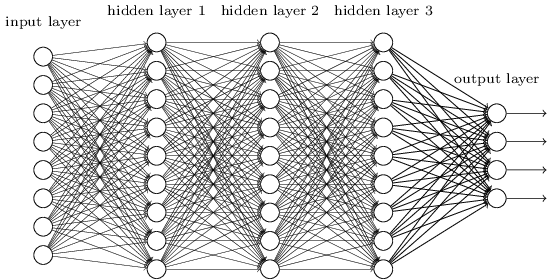
\includegraphics[width=0.50\textwidth]
	{pics/dnn.png}
	\caption{Contoh Arsitektur Deep Neural Netowork.}
	\label{fig:dnn}
\end{figure}

Karena arsitekturnya yang sederhana, DNN pada banyak kasus memiliki performa yang tidak sebaik arsitektur-arsitektur lain. DNN lebih tepat digunakan untuk melakukan tugas-tugas prediksi sederhana yang fitur-fitur dari data yang akan diprediksi sudah diketahui.

Convolutional Neural Network (CNN) merupakan arsitektur \deeplearning yang sering digunakan dalam bidang pengolahan citra. CNN pada umumnya terdiri dari beberapa convolution layer, pooling layer, dan fully-connected layer. Convolution layer dan Pooling layer merupakan beberapa jenis layer pada arsitektur ini yang tidak terdapat pada arsitektur-arsitektur lain. Convolution layer biasanya berfungsi untuk mengekstrak fitur-fitur dari data dua dimensi atau tiga dimensi yang masuk. Sedangkan pooling layer berfungsi mereduksi ukuran data output dari convolution layer dengan cara melakukan sampling terhadap data tersebut. Fully-connected layer diletakkan pada akhir arsitektur yang memiliki fungsi untuk melakukan prediksi, sama seperti DNN, dengan menggunakan fitur-fitur hasil ekstraksi convolution layer. Gambar merupakan contoh arsitektur CNN.

\begin{figure}
	\centering
	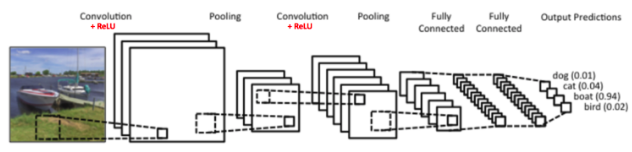
\includegraphics[width=0.50\textwidth]
	{pics/cnn.png}
	\caption{Contoh Arsitektur \conv \nn.}
	\label{fig:cnn}
\end{figure}


Recurrent Neural Network (RNN) merupakan arsitektur Deep Learning yang dapat memproses data yang bersifat sekuensial. Arsitektur ini terdiri dari input layer, hidden layer, dan output layer yang mengandung loop, dimana hasil prediksi dari output layer pada suatu waktu digunakan untuk mengubah parameter dari layer-layer sebelumnya untuk melakukan prediksi pada waktu berikutnya. Dapat dikatakan bahwa output dari suatu layer pada suatu waktu bergantung pada output dari layer itu sendiri pada waktu-waktu sebelumnya. Gambar merupakan contoh arsitektur RNN.

\begin{figure}
	\centering
	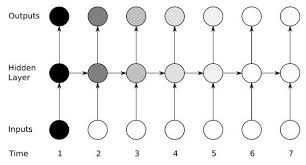
\includegraphics[width=0.50\textwidth]
	{pics/rnn.jpeg}
	\caption{Contoh Arsitektur Recurrent Neural Netowork.}
	\label{fig:rnn}
\end{figure}

RNN sangat populer dalam bidang Natural Language Processing (NLP) karena kemampuannya mengolah bahasa baik berupa audio atau teks. Hal ini karena bahasa berupa teks atau audio merupakan data yang bersifat sekuensial. 

Dengan melihat contoh-contoh arsitektur \deeplearning di atas, sekilas dapat diketahui bahwa Deep Learning memiliki beban komputasi yang cukup besar, terutama pada CNN, karena melibatkan banyak parameter dan banyak layer. Oleh karena itu, penggunaan CPU saja dirasa kurang cukup dalam menjalankan operasi-operasi pada Deep Learning.
%-----------------------------------------------------------------------------%
\section{Deep Learning Training dan Inference}
%-----------------------------------------------------------------------------%
Sama seperti \nn biasa, arsitektur \nn dalam Deep Learning memiliki parameter \weight pada setiap layer yang digunakan untuk menghitung skor dari input yang masuk ke suatu \layer dan meneruskan hasilnya ke \layer berikutnya. Deep Learning terdiri dari dua  tahap yaitu training dan inference. Pada tahap training, model \nn dilatih menggunakan sekumpulan data. Dalam hal ini yang dilatih adalah parameter \weight hingga menemukan parameter yang optimal.

Untuk mengawali proses \training, \weight awal diberikan terlebih dahulu kepada model. Biasanya \weight awal ini merupakan angka-angka acak berdasarkan suatu distribusi tertentu. Kemudian, model dengan \weight awal yang belum optimal tersebut digunakan untuk melakukan prediksi label atau skor dari data dengan melakukan \textit{forward pass} sepanjang model dari \layer pertama (input \layer) hingga mencapai \layer terakhir (\outputa \layer).

Hasil prediksi kemudian dibandingkan dengan label aslinya. Nilai \error dari prediksi dapat dihitung menggunakan fungsi tertentu, misalnya \textit{Mean Square Error}. Informasi \error ini kemudian dikirim kembali ke \layer-\layer sebelumnya dan akan digunakan oleh \layer-\layer terebut untuk memperbarui parameter \weight yang belum optimal tadi berdasarkan informasi \error yang diterima. \textit{Weight} dapat diperbarui menggunakan algoritma atau fungsi pembaruan \weight tertentu. Proses prediksi dan mengembalikan \error ke belakang ini disebut \textit{back propagation}. 

Setelah \training selesai, model \nn dapat digunakan untuk melakukan proses \inference. Tahap \inference merupakan tahap dimana model yang telah dilatih digunakan untuk melakukan prediksi. Proses prediksi ini sama dengan prediksi ketika melakukan \training yaitu dengan melakukan \textit{forward-pass} terhadap input data mulai dari \inputa \layer hingga \outputa \layer pada model. 

Letak perbedaan proses \inference dan \training pada \deeplearning adalah pada tahap \textit{back-propagation}. Setelah melakukan prediksi pada proses \inference , tidak lagi dilakukan \textit{back-propagation} terhadap \error hasil prediksi seperti pada proses \training. Hal ini karena tujuan dari \inference adalah mendapatkan hasil prediksi skor atau label yang dikeluarkan oleh model yang telah dilatih. Gambar 2.1 menunjukkan perbedaan proses \training dan \inference pada \nn . Terlihat bahwa \training melakukan pemrosesan data pada dua arah, sedangkan \inference hanya satu arah.

\begin{figure}
	\centering
	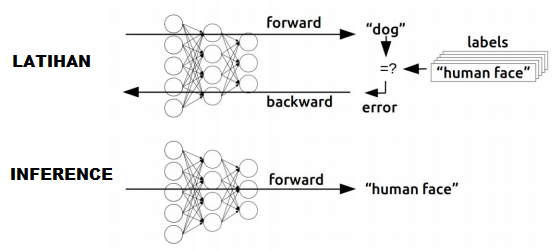
\includegraphics[width=0.50\textwidth]
	{pics/trainingvsinference.png}
	\caption{Perbedaan proses \training dan \inference pada \deeplearning.}
	\label{fig:trainvsinfer}
\end{figure}

\section{Operasi-operasi Deep Learning Inference}
%-----------------------------------------------------------------------------%
Tahap inference pada Deep Learning melibatakan banyak sekali operasi matriks yang biasanya merupakan operasi antara input data pada suatu layer dengan weight pada layer itu. Beberapa operasi bahkan memiliki kompleksitas yang tinggi. Berikut adalah beberapa contoh operasi penting yang sering muncul pada Deep Learning inference.

\subsection{Perkalian Matriks}
Operasi perkalian matriks pada Deep Learning inference merupakan salah satu operasi yang memiliki beban komputasi terbesar. Perkalian matriks dapat terjadi pada bagian fully-connected layer. Pada suatu fully-connected layer ke-l, parameter weight disimpan dalam bentuk matriks yang berukuran MxN dimana M adalah banyaknya node pada layer ke-l dan N adalah banyaknya node pada layer ke-(l-1). Baris ke-i pada weight matriks dari layer ke-l tersebut merupakan weight dari node ke-i pada layer ke-l. Untuk menentukan nilai node-node pada layer ke-l, matrix MxN tersebut dikalikan dengan matrix Nx1 yang berisi nilai-nilai node layer ke-(l-1) sehingga menghasilkan matriks Mx1. Kemudian activation function diterapkan terhadap setiap elemen matriks Mx1 tersebut dan kemudian bias juga ditambahkan jika ada sehingga menghasilkan matriks Mx1 yang merupakan nilai node-node layer ke-i. Gambar adalah ilustrasi dari operasi perkalian matriks pada fully-connected layer.

\begin{figure}
	\centering
	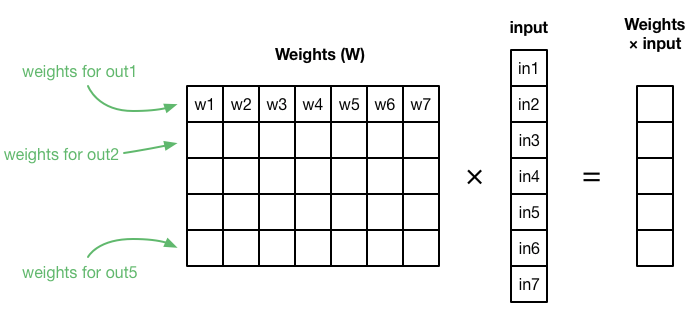
\includegraphics[width=0.50\textwidth]
	{pics/matmul.png}
	\caption{Perkalian matriks pada fully-connected layer saat mengalikan weight dengan input.}
	\label{fig:matmul}
\end{figure}

\subsection{Konvolusi Matriks}
Operasi konvolusi terjadi pada convolution layer dari CNN. Konvolusi merupakan penerapan filter atau kernel terhadap suatu input dengan mengkonvolusikan kernel tersebut terhadap input sehingga menghasilkan output. Input dan output suatu convolution layer merupakan matriks 3 dimensi yang merepresentasikan lebar, tinggi, dan kedalaman (biasa disebut channel). Sementara filter dinyatakan dalam matriks 4 dimensi yang merepresentasikan lebar filter, tinggi filter, kedalaman filter, dan banyaknya filter. Ukuran tinggi dan lebar filter selalu lebih kecil atau sama dengan tinggi dan lebar intput, sedangkan kedalamannya harus sama dengan kedalaman input.

Pada saat melakukan konvolusi terhadap input, masing-masing elemen pada suatu filter dikalikan dengan masing-masing elemen matriks input yang bersesuaian dengan posisi filter tersebut (seperti dot product pada vector) pada suatu waktu. Hasil dari satu kali operasi tersebut merupakan satu elemen dari matriks output pada posisi yang bersesuaian. Sehingga, setelah proses konvolusi selesai untuk satu filter, akan terbentuk satu lapis output dua dimensi. Jika semua filter sudah diterapkan maka akan terbentuk output tiga dimensi dengan kedalaman sesuai dengan banyaknya filter.

Gambar adalah contoh operasi konvolusi dengan input berukuran 5x5x1 dan filter berukuran 3x3x1.

\begin{figure}
	\centering
	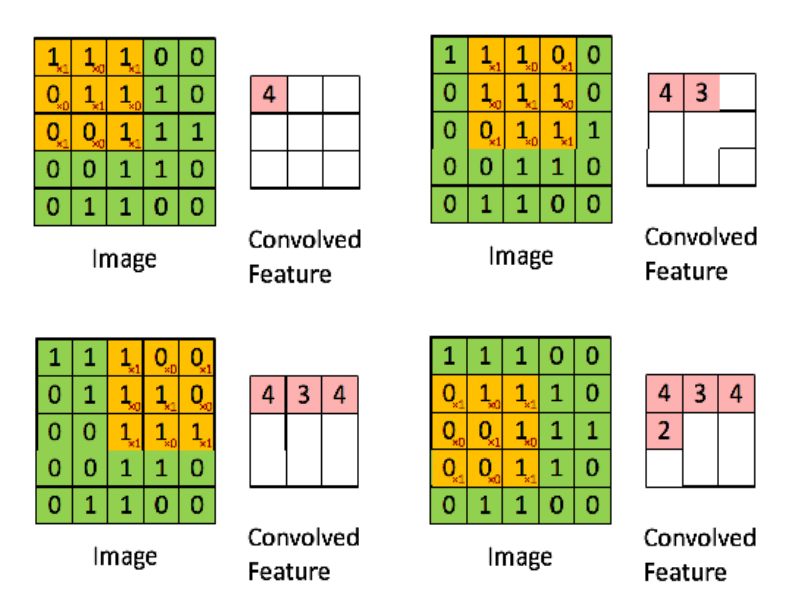
\includegraphics[width=0.50\textwidth]
	{pics/conv.png}
	\caption{Contoh Operasi Konvolusi. Image merupakan gambar masukan, convolved feature merupakan keluaran dari konvolusi.}
	\label{fig:conv}
\end{figure}

Pada operasi konvolusi dengan input berukuran MxNxD dan filter berukuran M'xN'xD' dan banyak filter adalah K, maka kompleksitas operasi konvolusi adalah O(MM'NN'DK). Operasi ini memiliki kompleksitas yang paling tinggi diantara layer-layer lain. 

\subsection{Transpose Matriks}
Transpose matriks dapat terjadi sebelum dilakukan perkalian matriks pada fully-connected layer. Operasi ini merupakan operasi membalik matriks terhadap diagonalnya. Pada matriks A dengan ukuran MxN, transpose dari A yaitu A' merupakan matriks yang tersusun dari elemen-elemen matriks A dimana A'ji = Aij untuk setiap bilangan bulat i dan j dimana 0 <= i < M dan 0 <= j < N. Gambar merupakan contoh operasi matriks transpose.

\begin{figure}
	\centering
	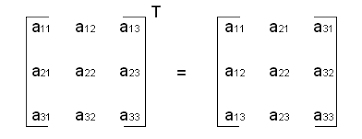
\includegraphics[width=0.50\textwidth]
	{pics/transpose.png}
	\caption{Transpose matrix pada \deeplearning \inference.}
	\label{fig:transpose}
\end{figure}

Matriks transpose memiliki kompleksitas O(MN).

\subsection{Penjumlahan Matriks}
Penjumlahan matriks dapat terjadi ketika melakukan penambahan bias terhadap hasil dari activation function suatu layer. Penjumlahan matriks dilakukan pada dua matriks berukuran sama. Pada dua matriks A dan B yang berukuran MxN, hasil penjumlahan matriks C merupakan matriks MxN dimana Cij = Aij + Bij untuk setiap bilangan bulat i dan j dimana 0 <= i < M dan 0 <= j < N. Gambar menunjukkan contoh operasi penjumlahan matriks.

\begin{figure}
	\centering
	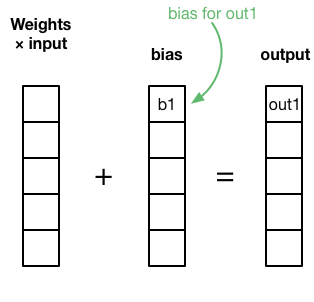
\includegraphics[width=0.50\textwidth]
	{pics/add.png}
	\caption{Penjumlahan matriks pada fully-connected layer saat menambahkan bias.}
	\label{fig:add}
\end{figure}

Pada kasus penambahan bias, lebar matriks biasanya adalah 1 atau bisa disebut sebagai vektor. Operasi ini memiliki kompleksitas O(MN), sama seperti matriks traspose.


\section{Tensorflow}
%-----------------------------------------------------------------------------%
Tensorflow merupakan perangkat lunak \textit{open-source} yang digunakan untuk komputasi numerik menggunakan representasi graf yang membentuk serangkaian operasi. Node pada graf merepresentasikan suatu operasi sedangkan edge mereperesentasikan tensor atau multidimensional array yang merupakan input atau output dari suatu operasi. Tensorflow dibuat oleh Google yang sejak awal digunakan untuk mendukung penelitian pada bidang \ml dan Deep Learning. Saat ini Tensorflow sudah sangat dikenal sebagai salah satu \framework \ml dan \deeplearning yang memiliki banyak fitur dan mudah dioperasikan. Salah satu fitur dari Tensorflow yang saat ini cukup menarik banyak perhatian adalah adanya dukungan untuk perangkat \textit{mobile} melalui \textit{library} Tensorflow Mobile dan Tensorflow Lite yang digunakan pada penelitian ini.

Tensorflow dan Tensorflow Lite diimplementasikan menggunakan bahasa C++ sehingga memungkinkan diterapkkannya OpenCL code. Kode sumber dari operasi-operasi \deeplearning \inference pada Tensorflow Lite terpisah dari kode sumber operasi-operasi \deeplearning \inference pada core Tensorflow. Modifikasi kode sumber Tensorflow Lite dengan menambahkan OpenCL code tidak akan mengubah behaviour dari program Tensorflow utama.

\section{Tensorflow Lite}
%-----------------------------------------------------------------------------%
Tensorflow Lite merupakan salah satu library dari Tensorflow yang dapat digunakan untuk proses \deeplearning \inference pada perangkat \mobile. Tensorflow sebenarnya memiliki dua \library yang dapat digunakan untuk melakukan Deep Learning \inference pada perangkat mobile, yaitu Tensorflow Mobile dan Tensorflow Lite. Tensorflow Lite memungkinkan proses inference pada perangkat mobile hanya untuk dua jenis model Neural Network yaitu Convolutional Neural Network. Tensorflow Lite, yang dirilis pada November 14, 2017, merupakan versi perbaikan dari Tensorflow Mobile yang telah dirilis terlebih dahulu.

Dalam menjalankan Deep Learning inference, Tensorflow Lite menerima input sebuah file .tflite yang berisi model dari Neural Network yang telah dilatih. Model file ini sebenarnya merupakan graph operasi Tensorflow yang berisi serangkaian node dan edge dengan ekstensi .pb namun telah dikonversi ke .tflite menggunakan Tensorflow Lite Converter. Model file tersebut diload oleh C++ API untuk kemudian diteruskan ke interpreter. API ini tersedia untuk perangkat Android maupun iOS. 

Interpreter mengeksekusi model menggunakan serangkaian kernel yang diload secara selektif, artinya hanya kernel yang berhubungan dengan operasi-operasi pada Model File saja yang diload. Ketika Tensorflow Lite dijalankan pada perangkat Android, ia akan menggunakan Android Neural Network API untuk meningkatkan performa inference. Namun tidak semua perangkat Android mendukung penggunaan Android Neural Network API. Gambar merupakan ilustrasi dari arsitektur Tensorfow Lite.

\begin{figure}
	\centering
	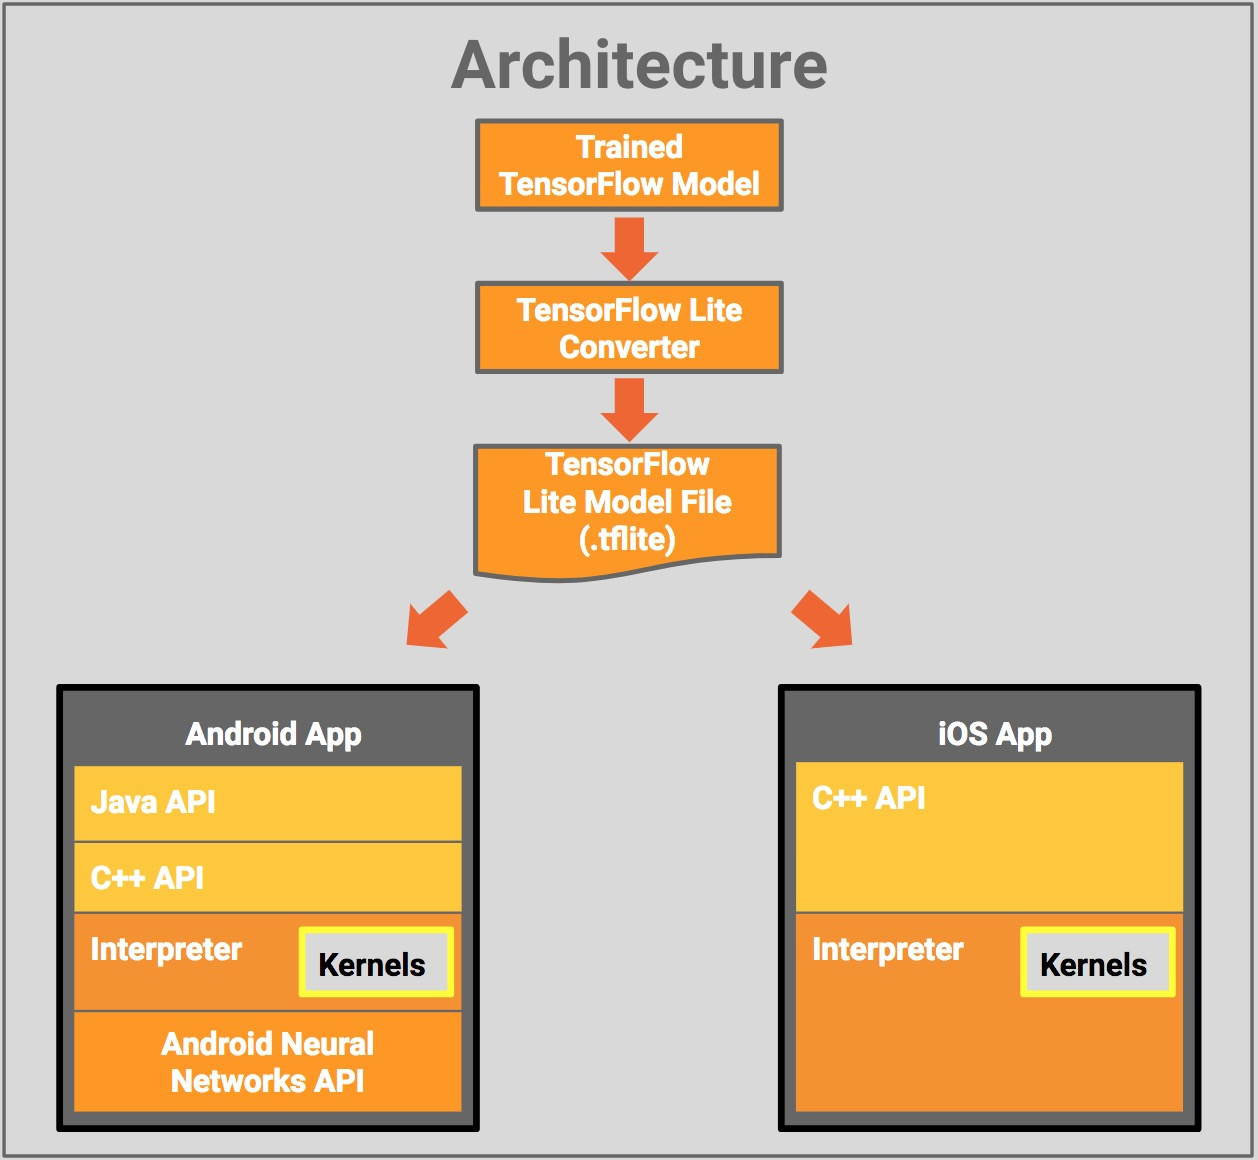
\includegraphics[width=0.50\textwidth]
	{pics/tflite.jpg}
	\caption{Ilustrasi dari arsitektur Tensorflow Lite.}
	\label{fig:tflite}
\end{figure}

Dibandingkan dengan Tensorflow Mobile, Tensorflow Lite telah mendapatkan berbagai macam optimisasi di dalamnya, sehingga memiliki performa yang lebih baik dari Tensorflow Mobile. Beberapa bug yang ada pada Tensorflow Mobile juga telah diperbaiki pada Tensorlfow Lite. Selain itu, fitur-fitur yang ditawarkan Tensorflow Lite juga lebih banyak dibandingkan Tensorflow Mobile.
Berikut adalah beberapa keunggulan Tensorflow Lite dibandingkan Tensorflow Mobile.

\begin{enumerate}
	\item Memiliki fitur yang dapat memprune node dari operation graph yang tidak terpakai pada proses inference.
	\item Memiliki kernel yang mendukung komputasi dalam 8-bit fixed point.
	\item Optimasi performa untuk operasi floating point maupun fixed point.
	\item Menggunakan pre-fused activation pada model Deep Learning.
	\item Memuat kernel secara selektif. Hanya yang terkait operasi-operasi pada model saja yang dimuat.
\end{enumerate}

\section{OpenCL}
%-----------------------------------------------------------------------------%
OpenCL merupakan antarmuka yang digunakan untuk pemrograman paralel pada prosesor yang berbeda-beda (CPU, GPU, dll) pada komputer, server, atau perangkat mobile. 
OpenCl dikenal dapat meningkatkan performa komputasi secara signifikan dengan menjalankan program secara paralel dan pada prosesor yang berbeda-beda.
Pada OpenCL terdapat dua sisi program, yaitu host dan device. Program device merupakan program yang dijalankan pada processor device yang ditargetkan (CPU, GPU, dll). Sementara itu program host berfungsi untuk mengatur jalannya program device, mulai dari menginisialisasi konteks, membuat program pada device, menyalin nilai variable dari host ke device memory, menjalankan kernel, dan mengambil nilai hasil komputasi dari device memory. Program host menggunakan bahasa C++ dengan beberapa ekstensi berupa fungsi dan tipe data khusus OpenCL.

Program yang dijalankan pada device terdiri dari satu atau lebih kernel. Kernel ditulis menggunakan bahasa C dengan sedikit perbedaan dari bahasa C biasa. Kernel pada OpenCl memiliki beberapa fungsi ekstensi dari bahasa C biasa, misalnya fungsi yang digunakan untuk mengambil worker ID dari suatu proses. 
Kernel ditulis sebagai string agar bisa digunakan oleh program host. Untuk dapat menjalankan program device, host harus terlebih dahulu membuat context. Context sendiri terbentuk dari satu atau lebih device. Contexts digunakan oleh OpenCL runtime untuk mengelola objek-objek seperti command-queues, memory, program, dan kernel. Context juga digunakan untuk mengeksekusi kernel-kernel pada satu atau lebih device yang telah terdefinisi pada context tersebut.

Setelah context terbentuk, host perlu membuat objek-objek lain seperti buffer dan command queue. Buffer merupakan bagian tertentu dari device memory yang digunakan untuk membaca atau menulis nilai yang diperlukan dalam proses kernel. Suatu buffer dapat bersifat read only, write only, atau read and write. Command queue merupakan antrian yang digunakan untuk menaruh perintah-perintah dari host kepada device. Contoh perintah adalah perintah untuk menjalankan kernel, perintah untuk menulis nilai ke buffer, dan perintah untuk membaca nilai dari buffer. Buffer dan command queue diinisialisasi pada bagian host. Gambar mengilustrasikan bagaimana OpenCL bekerja.

\begin{figure}
	\centering
	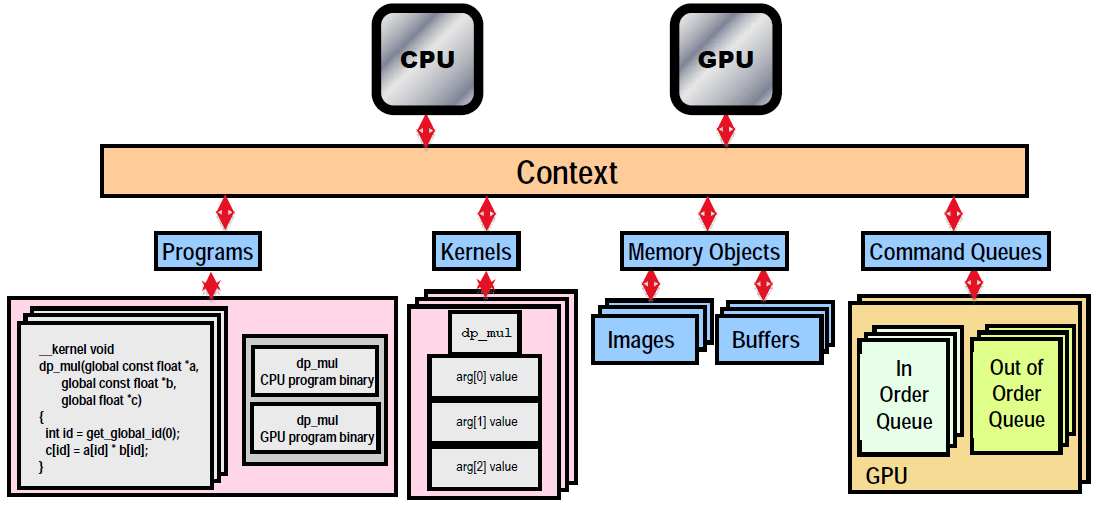
\includegraphics[width=0.50\textwidth]
	{pics/opencl-context.png}
	\caption{Cara kerja OpenCL.}
	\label{fig:context}
\end{figure}

OpenCL dapat digunakan pada perangkat yang memiliki library OpenCL, biasanya bernama libOpenCl.so. Pada NVidia GPU, library dapat diperoleh dalam paket installasi CUDA. Sedangkan pada perangkat android, beberapa vendor GPU seperti Qualcomm menyertakan library OpenCL pada perangkat mereka. Library libOpenCl.so ini biasanya terletak pada direktori /system/vendor/lib/. Berikut adalah contoh program host dan device (kernel) pada OpenCL.

\begin{lstlisting}[frame=single]
/* OpenCL Host Example */
void clHello() {
    cl_device_id device_id = NULL;
    cl_context context = NULL;
    cl_command_queue command_queue = NULL;
    cl_mem memobj = NULL;
    cl_program program = NULL;
    cl_kernel kernel = NULL;
    cl_platform_id platform_id = NULL;
    cl_uint ret_num_devices;
    cl_uint ret_num_platforms;
    cl_int ret;

    char string[MEM_SIZE];

    /* Get Platform and Device Info */
    ret = clGetPlatformIDs(1, &platform_id, 
    &ret_num_platforms);
    ret = clGetDeviceIDs( platform_id, 
    CL_DEVICE_TYPE_DEFAULT, 1, &device_id, 
    &ret_num_devices);

    /* Create OpenCL context */
    context = clCreateContext( NULL, 1, &device_id, 
    NULL, NULL, &ret);

    /* Create Command Queue */
    command_queue = clCreateCommandQueue(context, 
    device_id, 0, &ret);

    /* Create Memory Buffer */
    memobj = clCreateBuffer(context, 
    CL_MEM_READ_WRITE,MEM_SIZE * sizeof(char), NULL, 
    &ret);

    /* Create Kernel Program from the source */
    program = clCreateProgramWithSource(context, 1, 
    (const char **)&CLCL_HELLO,
    NULL, &ret);

    /* Build Kernel Program */
    ret = clBuildProgram(program, 1, &device_id, NULL, 
    NULL, NULL);

    /* Create OpenCL Kernel */
    kernel = clCreateKernel(program, "hello", &ret);

    /* Set OpenCL Kernel Arguments */
    ret = clSetKernelArg(kernel, 0, sizeof(cl_mem), 
    (void *)&memobj);

    /* Execute OpenCL Kernel */
    ret = clEnqueueTask(command_queue, kernel, 0, 
    NULL,NULL);

    /* Copy results from the memory buffer */
    ret = clEnqueueReadBuffer(command_queue, memobj, 
    CL_TRUE, 0,
    MEM_SIZE * sizeof(char),string, 0, NULL, NULL);

    /* Display Result */
    __android_log_print(ANDROID_LOG_DEBUG, "OpenCL", 
    "Hello: %s", string);


    /* Finalization */
    ret = clFlush(command_queue);
    ret = clFinish(command_queue);
    ret = clReleaseKernel(kernel);
    ret = clReleaseProgram(program);
    ret = clReleaseMemObject(memobj);
    ret = clReleaseCommandQueue(command_queue);
    ret = clReleaseContext(context);
}
\end{lstlisting}

\begin{lstlisting}[frame=single]
/* OpenCL kernel example */
const char *CLCL_HELLO =
    "__kernel void hello(__global char* string)\n"
    "{\n"
    "   string[0] = 'H';\n"
    "   string[1] = 'e';\n"
    "   string[2] = 'l';\n"
    "   string[3] = 'l';\n"
    "   string[4] = 'o';\n"
    "   string[5] = '\\0';\n"
    "}\n"
    "";
\end{lstlisting}

\section{OpenCL Data Parallelism}
%-----------------------------------------------------------------------------%
OpenCL mendukung pemrograman paralel yang dapat dilakukan pada level data maupun level device. Ketika suatu program hanya dijalankan pada satu device saja, misalnya pada penelitian ini yang hanya menggunakan rGPU sebagai OpenCL device, paralelisasi tetap dapat dilakukan pada level data. Maksudnya, data yang diproses dipecah-pecah sehingga masing-masing unit pemrosesan hanya memproses sebagian dari data secara independen terhadap unit pemrosesan lainnya. Hal ini salah satunya dapat dilakukan pada operasi matriks, misalnya pada penjumlahan matriks, penambahan elemen-elemen matriks dapat dilakukan secara paralel dengan masing-masing unit pemrosesan hanya memproses elemen pada baris dan kolom yang sama saja.

Dalam OpenCL, unit pemrosesan ini disebut dengan work item. Setiap work item melakukan hal yang sama namun hanya datanya saja yang berbeda. Dengan kata lain, setiap work item menjalankan kernel yang sama. Masing-masing work item memiliki private memory. Setiap work item juga memiliki ID masing-masing yang dapat berupa ID secara global maupun ID work item itu dalam suatu grup tertentu. ID bilangan bulat positif yang dimulai dari 0.  

Beberapa work item dapat membentuk work/local group. Proses yang terjadi pada suatu work group dapat melakukan sinkronisasi. Selain itu, work group memiliki memory tersendiri yang disebut local memory. Memory ini merupakan shared memory dimana setiap work item dalam grup dapat menggunakan local memory tersebut bersamaan. Work group juga memiliki ID seperti work item. Gambar merupakan ilustrasi dari work item dan work group pada OpenCL.

\begin{figure}
	\centering
	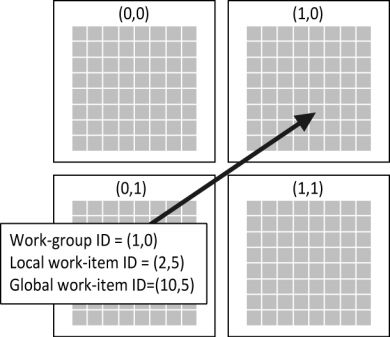
\includegraphics[width=0.50\textwidth]
	{pics/opencl-work.jpg}
	\caption{OpenCL work group dan work ite.}
	\label{fig:work}
\end{figure}

Saat suatu proses berjalan pada device, kita dapat mengambil ID dari work item atau work group yang menjalankan proses tersebut. Dengan demikian kita dapat mengatur suatu work item atau work group harus memproses bagian mana saja dari data. Misalnya dalam penjumlahan vektor, work item dengan ID i hanya memproses elemen ke i dari vektor-vektor yang dijumlahkan.
%-----------------------------------------------------------------------------%
\chapter{\babTiga}
%-----------------------------------------------------------------------------%
Pada bagian ini akan dijelaskan metodologi yang digunakan dalam penelitian. Metodologi ini mencakup metode implementasi OpenCL untuk masing-masing operasi serta metode eksperimen.

\section{Metode Implementasi }
%-----------------------------------------------------------------------------%
Pada penelitian ini penulis memanfaatkan Tensorflow Lite untuk menjalankan \textit{Deep Learning inference} pada perangkat \textit{mobile}. Tensorflow Lite memiliki \textit{kernel} tersendiri yang terpisah dari \textit{core} Tensorflow.  Penulis memodifikasi Tensorflow Lite \textit{kernel} dengan menambahkan implementasi OpenCL untuk operasi perkalian matriks-matriks, perkalian matriks-vektor, dan konvolusi matriks sehingga operasi-operasi tersebut dapat dijalankan pada GPU ketika \textit{inference} berlangsung. Implementasi OpenCL pada tiga operasi tersebut hanya dapat digunakan oleh \textit{fully-connected} layer dan \textit{convolution layer}.

Tensorflow Lite telah memiliki dua jenis Tensorflow Lite \textit{kernel} untuk operasi matriks pada \textit{convolution layer} dan \textit{fully-connected layer}, yaitu \textit{naive kernel} dan \textit{optimized kernel}, dimana keduanya dijalankan pada CPU. Dengan menambahkan Tensorflow Lite \textit{kernel} yang diimplementasikan melalui OpenCL, ada tiga jenis Tensorflow Lite \textit{kernel} yang dapat digunakan. Saat kompilasi, pengguna dapat memilih untuk menggunakan \textit{naive kernel} (CPU), \textit{optimized kernel} (CPU), atau OpenCL \textit{kernel} (GPU). \pic~\ref{fig:modifieddiagram} menunjukkan bagaimana penulis memodifikasi Tensorflow Lite \textit{kernel}.

\begin{figure}
	\centering
	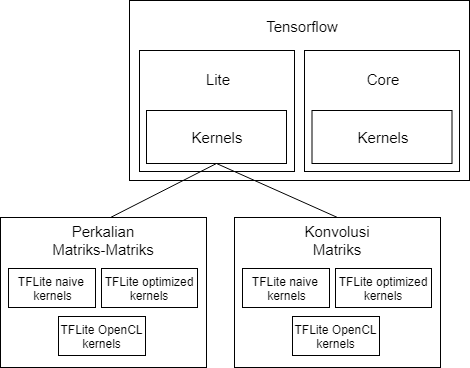
\includegraphics[width=0.50\textwidth]
	{pics/modifieddiagram.png}
	\caption{Modifikasi Tensorflow Lite \textit{kernel} dengan menambahkan satu jenis \textit{kernel} baru untuk operasi perkalian matriks-matriks dan konvolusi matriks yang diimplementasikan melalui OpenCL dan berjalan di GPU.}
	\label{fig:modifieddiagram}
\end{figure}

Persiapan-persiapan OpenCL seperti yang disebutkan pada BAB II memerlukan cukup banyak waktu. Untuk mengurangi biaya persiapan yang mahal, beberapa persiapan tidak dilakukan pada setiap \textit{inference}, namun hanya dilakukan satu kali pada awal berjalannya aplikasi \textit{Deep Learning}. Hal ini dilakukan dengan cara meletakkan persiapan-persiapan tersebut pada \textit{interpreter} sehingga persiapan tersebut hanya dilakukan ketika Tensorflow Lite melakukan interpretasi model. Objek-objek hasil dari persiapan OpenCL seperti \textit{context} dan \textit{buffer} tersebut kemudian dapat diberikan sebagai argumen ketika melakukan interpretasi \textit{fully-connected layer} dan \textit{convolution layer}. Ketika \textit{inference}, objek \textit{fully-connected layer} dan \textit{convolution layer} pada Tensorflow Lite dapat menggunakan objek-objek OpenCL yang telah dipersiapkan di awal. Persiapan untuk OpenCL yang dilakukan pada awal berjalannya aplikasi dapat dilihat pada \tab~\ref{tab:SetupCL}.

\begin{table}
	\centering
	\caption{Persiapan OpenCL yang dilakukan satu kali pada awal berjalannya aplikasi.}
	\label{tab:SetupCL}
	\begin{tabular}{| l | l |}
		\hline
		\textbf{No.} & \textbf{Persiapan OpenCL} \\ 
		\hline
		1 & Membuat \textit{context} \\ 
		\hline 
		2 & Membuat \textit{command queue} \\ 
		\hline 
		3 & Membuat \textit{kernel} \\ 
		\hline
		4 & Membuat \textit{buffer} \\ 
		\hline
	\end{tabular}
\end{table}

Persiapan yang tidak dapat dilakukan hanya satu kali adalah menyalin data masukan operasi \textit{inference} dari memori CPU ke memori GPU. Proses menyalin data ini harus dikerjakan pada setiap \textit{inference} karena data masukan bersifat dinamis. Perhatikan \pic~\ref{fig:initcl} dan \pic~\ref{fig:copydata} untuk mengetahui lebih jelas bagaimana persiapan untuk OpenCL dilakukan pada penelitian ini.

\begin{figure}
	\centering
	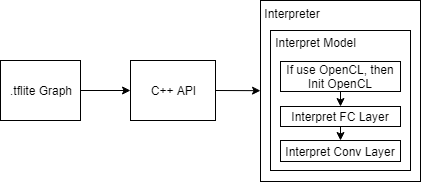
\includegraphics[width=0.50\textwidth]
	{pics/initcl.png}
	\caption{Metode persiapan untuk OpenCL yang dilakukan hanya satu kali di awal berjalannya suatu aplikasi \textit{Deep Learning}. Persiapan dilakukan ketika \textit{interpreter} melakukan inisiasi model.}
	\label{fig:initcl}
\end{figure}

\begin{figure}
	\centering
	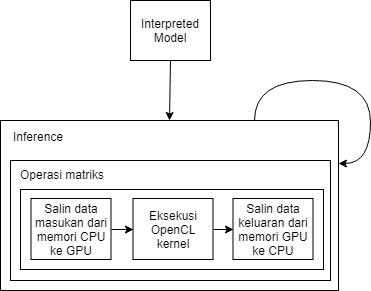
\includegraphics[width=0.50\textwidth]
	{pics/copydata.png}
	\caption{Proses menyalin data masukan dan keluaran antara memori CPU dan GPU dilakukan pada setiap \textit{inference}. Proses menyalin data tidak dapat dilakukan satu kali saja karena data bersifat dinamis.}
	\label{fig:copydata}
\end{figure}

\subsection{Metode Implementasi Konvolusi Matriks }
Operasi konvolusi matriks memiliki dua matriks masukan, yaitu \textit{image} dan \textit{filter}, dan satu matriks keluaran yaitu matriks \textit{output}. Matriks-matriks tersebut merupakan matriks empat dimensi yaitu kanal, baris, kolom, dan \textit{batch}. Seluruh matriks masukan dan keluaran disimpan di memori GPU secara linear dengan struktur seperti pada \pic~\ref{fig:linearconv}. Semua matriks menggunakan tipe data vektor $float4$. Apabila banyaknya kanal dari matriks bukan kelipatan empat, maka diberikan \textit{padding} pada struktur linear di memori GPU tersebut sedemikian sehingga setiap vektor $float4$ mengandung elemen-elemen yang merupakan elemen-elemen matriks pada kolom, baris, dan \textit{batch} yang sama. 

\begin{figure}
	\centering
	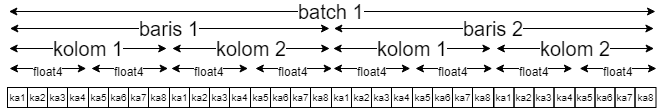
\includegraphics[width=0.50\textwidth]
	{pics/linearconv.png}
	\caption{Struktur linear matriks masukan dan keluaran yang disimpan di memori GPU untuk operasi konvolusi. Elemen ke-15 dari data linear tersebut adalah elemen pada kanal ke-7, kolom ke-2, baris ke-1 dan \textit{batch} ke-1 dari matriks.}
	\label{fig:linearconv}
\end{figure}

Misalkan banyaknya kanal, tinggi, lebar, dan banyaknya \textit{batch} dari \textit{image}, \textit{filter}, dan \textit{output} berturut-turut adalah $C_i \times H_i \times W_i \times B_i$, $C_f \times H_f \times W_f \times B_f$, dan $C_o \times H_o \times W_o \times B_o$. Pada implementasi ini digunakan \textit{work-space} dua dimensi berukuran $H_{ws} \times W_{ws}$ dan \textit{work-group} dua dimensi berukuran $H_{wg} \times W_{wg}$ dengan $H_{ws} = H_o' \times B_o$ dan $W_{ws} = W_o' \times ceil(C_o/4)$, dimana $Wo'$ adalah bilangan kelipatan $W_{wg}$ terkecil yang lebih besar atau sama dengan $W_o$ dan $H_o'$ adalah bilangan kelipatan $H_{wg}$ terkecil yang lebih besar atau sama dengan $H_o$. \pic~\ref{fig:wiconv} merupakan contoh struktur \textit{work-space} dengan $H_{wg} = 8$ dan $W_{wg} = 32$.

\begin{figure}
	\centering
	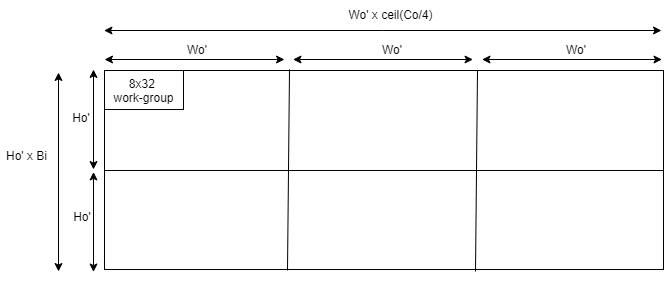
\includegraphics[width=0.50\textwidth]
	{pics/wiconv.png}
	\caption{Struktur \textit{work-space} untuk konvolusi matriks. Dalam kasus ini $W_o$ adalah kelipatan 32 dan $H_o$ adalah kelipatan 8.}
	\label{fig:wiconv}
\end{figure}

Dengan struktur tersebut, setiap vektor $float4$ pada matriks \textit{output} dikomputasi oleh suatu \textit{work-item} yang unik. Selain itu, suatu \textit{work-group} melakukan komputasi untuk memperoleh satu blok matriks \textit{output} dengan tinggi, lebar, dan banyaknya kanal $H_{wg} \times W_{wg} \times 4$. Blok tersebut merupakan hasil konvolusi dari suatu blok lain pada matriks \textit{image} dengan tinggi, lebar, dan banyaknya kanal $(H_{wg}+H_f-1) \times (W_{wg}+W_f-1) \times C_i$ dengan empat \textit{filter} yang berbeda. Ini dapat dilihat pada \pic~\ref{fig:convblock}.   

\begin{figure}
	\centering
	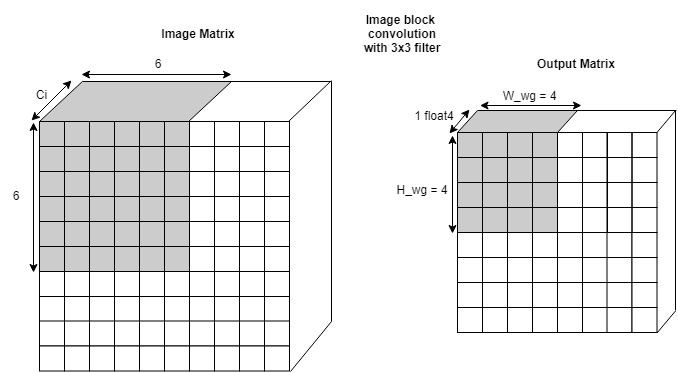
\includegraphics[width=0.50\textwidth]
	{pics/convblock.png}
	\caption{Blok pada matriks \textit{output} yang dikomputasi oleh suatu \textit{work-group}. Blok tersebut terdiri dari empat kanal. Blok berwarna abu-abu pada matriks \textit{output} merupakan hasil konvolusi dari blok abu-abu dari matriks \textit{image}.}
	\label{fig:convblock}
\end{figure}

Perhatikan bahwa untuk memperoleh satu blok matriks \textit{output}, hampir semua elemen pada blok matriks \textit{image} akan diakses lebih dari satu kali oleh \textit{work-group}. Mengetahui fakta ini, penulis menggunakan \textit{local memory caching} untuk mengurangi redundansi akses ke \textit{global memory}. Konvolusi untuk suatu blok matriks \textit{output} dilakukan dalam $ceil(C_i/4)$ iterasi, dimana setiap iterasi hanya melibatkan blok matriks \textit{image} yang berukuran $(H_{wg}+H_f-1) \times (W_{wg}+W_f-1) \times 4$ seperti yang dapat dilihat pada \pic~\ref{fig:conviter}. Hasil konvolusi dari semua iterasi kemudian diakumulasikan. Dengan menggunakan \textit{local memory caching}, pada setiap iterasi blok matriks \textit{image} ini disalin terlebih dahulu dari \textit{global memory} ke \textit{local memory} sebelum digunakan untuk komputasi. Setiap \textit{work-item} pada \textit{work-group} bertugas menyalin maksimal empat vektor $float4$ dari blok matriks \textit{image} ke \textit{local memory} seperti yang terlihat pada \pic~\ref{fig:convlocal}.  

\begin{figure}
	\centering
	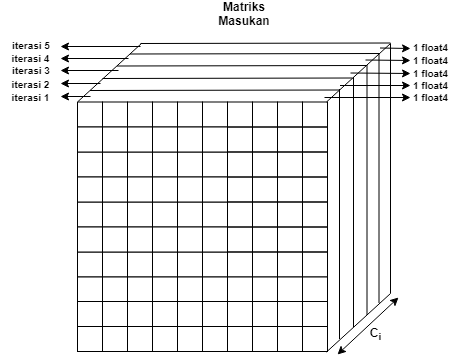
\includegraphics[width=0.50\textwidth]
	{pics/conviter.png}
	\caption{Operasi konvolusi dilakukan dalam $ceil(C_i/4)$ iterasi dimana $C_i$ adalah kedalaman \textit{image}. Setiap iterasi melibatkan blok matriks \textit{image} dengan kedalaman 4, sesuai dengan panjang vektor $float4$.}
	\label{fig:conviter}
\end{figure}

\begin{figure}
	\centering
	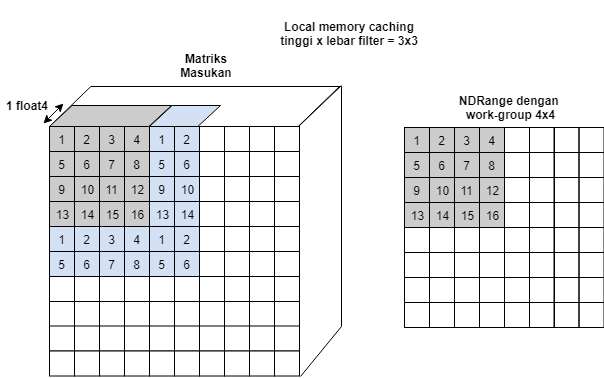
\includegraphics[width=0.50\textwidth]
	{pics/convlocal.png}
	\caption{\textit{Local memory cahing} terhadap matriks \textit{image} pada suatu iterasi dalam kasus \textit{filter} berukuran panjang dan lebar $3 \times 3$. \textit{Work-item} dengan nomor $i$ bertugas menyalin vektor-vektor $float4$ dari \textit{image} dengan nomor $i$ ke local memory.}
	\label{fig:convlocal}
\end{figure}

\subsection{Metode Implementasi Perkalian Matriks-Matriks }
Dalam pembahasan ini dimisalkan matriks masukan adalah matriks A dan matriks B, sedangkan matriks keluaran adalah matriks C. Sama seperti konvolusi, seluruh matriks disimpan secara linear di memori GPU. Matrix A dan matriks C disimpan secara \textit{row-major}, sedangkan matrix B disimpan secara \textit{column-major} seperti pada \pic~\ref{fig:linearmatmat}.  Semua matriks menggunakan tipe data vektor $float4$. Jika lebar dari matriks A atau C bukan kelipatan 4, maka diberikan \textit{padding} pada struktur linear di memori GPU sedemikian sehingga setiap vektor $float4$ mengandung elemen-elemen yang merupakan elemen-elemen matriks pada baris yang sama. Untuk matriks B, \textit{padding} diberikan jika tingginya bukan kelipatan 4.

\begin{figure}
	\centering
	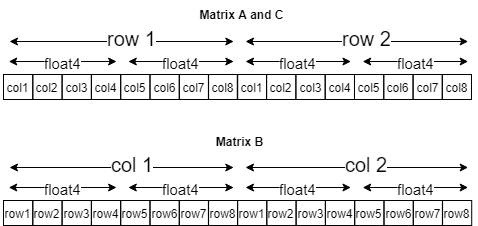
\includegraphics[width=0.50\textwidth]
	{pics/linearmatmat.png}
	\caption{Struktur linear matriks A, B, dan C pada operasi perkalian matriks-matriks. A dan C disimpan secara \textit{row-major}, sedangkan B secara \textit{column-major}.}
	\label{fig:linearmatmat}
\end{figure}

Misalkan matriks A berukuran $M \times K$ dan matriks B berukuran $K \times N$, maka matriks C berukuran $M \times N$. Untuk menjalankan operasi perkalian matriks-matriks di GPU, digunakan \textit{work-space} dua dimensi dengan ukuran $H_{ws} \times W_{ws}$ dan \textit{work-group} dua dimensi berukuran $H_{wg} \times W_{wg}$ dimana $H_{ws}$ adalah bilangan kelipatan $H_{wg}$ terkecil yang lebih besar atau sama dengan $M$ dan $W_{ws}$ adalah bilangan kelipatan $W_{wg}$ terkecil yang lebih besar atau sama dengan $ceil(N/4)$. Untuk ukuran \textit{work-group}, berlaku aturan $H_{wg} = 4 \times W_{wg}$. 

\begin{figure}
	\centering
	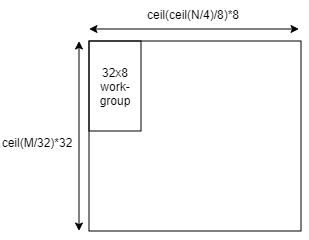
\includegraphics[width=0.50\textwidth]
	{pics/wimatmat.png}
	\caption{Struktur \textit{work-space} untuk perkalian matriks-matriks. Dalam kasus ini tinggi \textit{work-space} adalah kelipatan 32 dan lebarnya adalah kelipatan 8.}
	\label{fig:wimatmat}
\end{figure}

Dengan struktur di atas, setiap vektor $float4$ pada matriks C dikomputasi oleh satu \textit{work-item} yang unik. Lalu, masing-masing \textit{work-group} melakukan komputasi untuk memperoleh satu blok pada matriks C yang berukuran $H_{wg} \times H_{wg}$ seperti pada \pic~\ref{fig:wimatmat}. Perhatikan bahwa setiap blok matriks C tersebut diperoleh dari perkalian matriks antara dua blok lain, yaitu satu blok dari matriks A berukuran $H_{wg} \times K$ dan satu blok dari matriks B berukuran $K \times H_{wg}$. \pic~\ref{fig:blackmatmat} adalah contoh perkalian antara dua blok matriks untuk menghasilkan blok berukuran $32 \times 32$ pada matriks C ketika ukuran \textit{work-group} adalah $32 \times 8$.

\begin{figure}
	\centering
	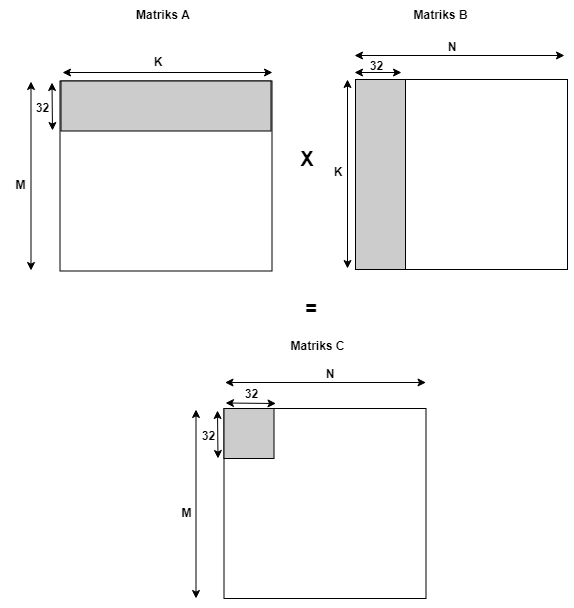
\includegraphics[width=0.50\textwidth]
	{pics/blockmatmat.png}
	\caption{Perkalian antara dua blok $32 \times K$ dan $K \times 32$ pada matriks A dan B sehingga menghasilkan satu blok $32 \times 32$ pada matriks C. Ukuran work-group dalam kasus ini adalah $32 \times 8$.}
	\label{fig:blockmatmat}
\end{figure}

Seperti pada konvolusi, perkalian dua blok matriks tersebut juga mengandung redundansi akses \textit{global memory} karena elemen-elemen yang sama pada blok diakses lebih dari satu kali. Penulis juga menggunakan \textit{local memory caching} dalam implementasi ini. Perkalian antar dua blok matriks A dan B dilakukan dalam $ceil(K/H_{wg})$ iterasi. Pada setiap iterasi, dilakukan perkalian dua blok yang berukuran lebih kecil yaitu antara blok $H_{wg} \times H_{wg}$ dari matriks A dengan blok $H_{wg} \times H_{wg}$ dari matriks B seperti pada \pic~\ref{fig:matmatiter}. Hasil perkalian dari semua iterasi kemudian diakumulasikan. Pada setiap iterasi, masing-masing \textit{work-item} pada \textit{work-group} berutgas menyalin dua vektor $float4$, satu dari blok matriks A dan satu dari blok matriks B, ke \textit{local memory} seperti yang terlihat pada \pic~\ref{fig:localmatmat} sebelum komputasi dilakukan.

\begin{figure}
	\centering
	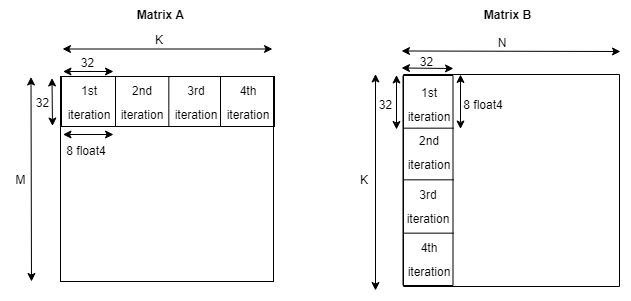
\includegraphics[width=0.50\textwidth]
	{pics/matmatiter.png}
	\caption{Operasi perklaian matriks-matriks yang dilakukan dalam $ceil(K/32)$ iterasi pada kasus ukuran work-group $32 \times 8$. Setiap iterasi melibatkan blok matriks A dengan lebar 32 dan blok matriks B dengan tinggi 32.}
	\label{fig:matmatiter}
\end{figure}

\begin{figure}
	\centering
	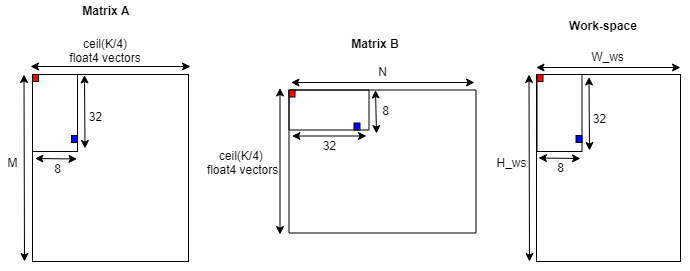
\includegraphics[width=0.50\textwidth]
	{pics/localmatmat.png}
	\caption{Pembagian kerja untuk menyalin blok matriks A dan B dari \textit{global memory} ke \textit{local memory} pada \textit{work-group} dengan ukuran $32 \times 8$. Masing-masing \textit{work-item} menyalin dua vektor $float4$. \textit{Work-item} merah memuat vektor berwarna merah dan \textit{work-item} biru memuat vektor berwarna biru.}
	\label{fig:localmatmat}
\end{figure}

\section{Metode Eksperimen }
%-----------------------------------------------------------------------------%
Eksperimen dilakukan terhadap masing-masing jenis Tensorflow Lite \textit{kernel} untuk operasi perkalian matriks-matriks dan konvolusi matriks, yaitu Tensorflow Lite \textit{naive kernel} yang berjalan di CPU, Tensorflow Lite \textit{optimized kernel} yang berjalan di CPU, dan Tensorflow Lite OpenCL \textit{kernel} yang berjalan di GPU. Dalam eksperimen ini penulis mengukur kecepatan eksekusi tiga \textit{kernel} tersebut pada berbagai kasus dan ukuran matriks atau vektor masukan. Hasil pengukuran kecepatan dari masing-masing \textit{kernel} kemudian dibandingkan. Untuk Tensorflow Lite OpenCL \textit{kernel}, penulis melakukan dua jenis pengukuran kecepatan. Pertama, pengukuran dilakukan terhadap eksekusi OpenCL \textit{kernel} saja (komputasi saja). Kedua, pengukuran dilakukan terhadap komputasi OpenCL beserta persiapan OpenCL yang diperlukan pada setiap \textit{inference}, yaitu proses menyalin data antar memori CPU dan GPU. Dengan demikian, penulis dapat mengetahui pada apakah \textit{bottleneck} dari OpenCL terletak pada transfer data antar memori atau terletak pada komputasi. Untuk menghitung kecepatan dari suatu Tensorflow Lite \textit{kernel} penulis menggunakan \textit{wall-clock time} dengan cara menghitung selisih dari \textit{wall-clock time} sebelum dan sesudah Tensorflow Lite \textit{kernel} berjalan.
%-----------------------------------------------------------------------------%
\chapter{\babEmpat}
%-----------------------------------------------------------------------------%
Bagian ini berisi penjelasan mengenai implementasi program-program yang terkait dengan penelitian. Program tersebut meliputi perkalian matriks, kovolusi matriks, transpose matriks, serta penjumlahan matriks yang diimplementasikan menggunakan OpenCL dan diintegrasikan ke Tensorflow Lite. 

%-----------------------------------------------------------------------------%
\section{OpenCL Matriks Multiplication}
%-----------------------------------------------------------------------------%
Ukuran blok yang digunakan disesuaikan dengan ukuran work-group yang disarankan pada OpenCL. Pada umunya perangkat android menyarankan ukuran kelipatan 8, sehingga ukuran blok dapat diambil 8x8, 16x32 atau 32x32. Ukuran lebih besar dari 32 tidak disarankan karena mayoritas perangkat memiliki batas jumlah work-item dalam suatu work-group sebanyak 1024 (32x32).
///////////

Implementasi perkalian matriks menggunakan blocking matrix multiplication. Kedua matriks yang dikalikan dibagi ke dalam beberapa block yang sama dimana satu block memiliki ukuran 32x32. Perhatikan pada gambar , terdapat dua matriks A dan B yang masing-masing berukuran MxK dan KxN. Dengan demikian perkalian keduanya menghasilkan matriks C yang berukuran MxN. Blok pada matriks C yang berwarna ungu diperoleh dari dua tahap perkalian matriks, yaitu perkalian antara blok hijau muda dan blok biru muda pada matriks A dan B kemudian ditambahkan dengan perkalian antara blok hijau tua dan blok biru tua pada matriks A dan B.

\begin{figure}
	\centering
	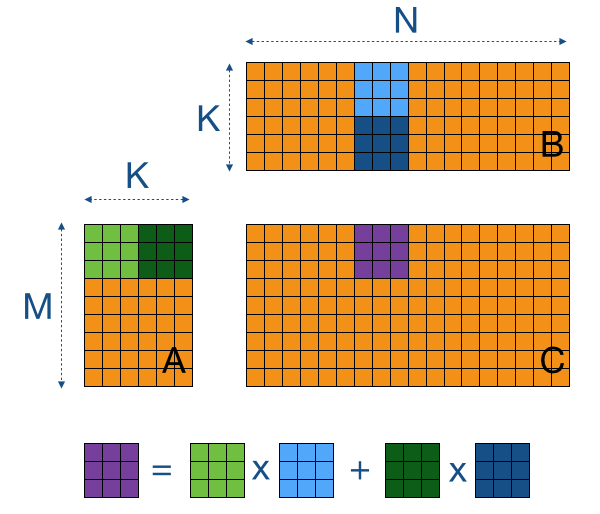
\includegraphics[width=0.50\textwidth]
	{pics/matmul-block1.png}
	\caption{Perkalian matriks per blok.}
	\label{fig:matmulblock}
\end{figure}

Motivasi dari penggunaan blok pada perkalian matriks adalah untuk meningkatkan efisiensi penggunaan cache pada GPU. Perhatikan bahwa untuk mendapatkan suatu elemen baris ke i dan kolom ke j dari matriks, baris ke i dari matriks A dan kolom ke j dari akan diload ke memory dan cache. Kemudian untuk mendapatkan suatu elemen baris ke i+1 dan kolom ke j dari matriks, kolom ke j dari matriks B kembali diload ke memory. Kolom ke j dari matriks B ini selalu digunakan ulang dalam menghitung elemen kolom ke j pada matriks C.

Untuk matriks berukuran besar, besar kemungkinan bahwa kolom tersebut sudah terhapus dari cache karena sebelum memproses kolom itu lagi, cache terlebih dahulu digunakan untuk menyimpan kolom-kolom lain karena sudah banyak perkalian yang dilakukan. Sedangkan ketika matriks berukuran kecil, peluang kolom tersebut masih berada di cache lebih tinggi, sehingga komputasi menggunakan kolom tersebut menjadi lebih cepat. Inilah mengapa matriks dibagi ke dalam beberapa bagian yang lebih kecil untuk dikalikan secara bertahap agar frekuensi penggunaan cache lebih tinggi sehingga komputasi lebih cepat. 

Perkalian per blok ini dapat diimplementasikan dalam OpenCL kernel seperti berikut. Iterasi dilakukan sebanyak K/blocksize kali. Pada setiap iterasi, perkalian per blok dilakukan untuk 32 kolom dari matriks A (semua baris) dan 32 baris dari matriks B (semua kolom). Ingat bahwa ukuran blok adalah 32x32.

\begin{lstlisting}[frame=single]
__kernel void matrixVectorMul(__global float* C, 
    const __global float* A, 
    const __global float* B, 
    int K, int M, int N) { 

	// Local row ID (max: 32)
    const int row = get_local_id(0);
    // Local col ID (max: 32)  
    const int col = get_local_id(1);
    // Row ID of C (0..M)  
    const int globalRow = 32*get_group_id(0) + row; 
    // Col ID of C (0..N) 
    const int globalCol = 32*get_group_id(1) + col;  

    __local float Asub[32][32]; 
    __local float Bsub[32][32]; 

    float acc = 0.0; 

    const int numTiles = ((K-1)/32)+1; 
    for (int t=0; t<numTiles; t++) { 

        const int tiledRow = 32*t + row; 
        const int tiledCol = 32*t + col; 
        if((tiledCol < K) && (globalRow < M)) {
            Asub[col][row] = A[globalRow*K + tiledCol]; 
        }  
        else {   
            Asub[col][row] = 0.0; 
        }  
        if((tiledRow < K) && (globalCol < N)) {
            Bsub[col][row] = B[globalCol*K + tiledRow]; 
        }  
        else {   
            Bsub[col][row] = 0.0; 
        }  

        barrier(CLK_LOCAL_MEM_FENCE); 

        for (int k=0; k<32; k++) { 
            acc += Asub[k][row] * Bsub[col][k]; 
        } 

        barrier(CLK_LOCAL_MEM_FENCE); 
    } 

    if((globalRow < M) && (globalCol < N)) { 
        C[globalCol*M + globalRow] = acc; 
    }
}
\end{lstlisting}

%-----------------------------------------------------------------------------%
\section{OpenCL Matriks Convolution}
%-----------------------------------------------------------------------------%

%-----------------------------------------------------------------------------%
\section{Vulkan Matriks Multiplication}
%-----------------------------------------------------------------------------%
Implementasi perkalian matriks menggunakan blocking matrix multiplication. Kedua matriks yang dikalikan dibagi ke dalam beberapa block yang sama dimana satu block memiliki ukuran 32x32. Perhatikan pada gambar , terdapat dua matriks A dan B yang masing-masing berukuran MxK dan KxN. Dengan demikian perkalian keduanya menghasilkan matriks C yang berukuran MxN. Blok pada matriks C yang berwarna ungu diperoleh dari dua tahap perkalian matriks, yaitu perkalian antara blok hijau muda dan blok biru muda pada matriks A dan B kemudian ditambahkan dengan perkalian antara blok hijau tua dan blok biru tua pada matriks A dan B.

\begin{figure}
	\centering
	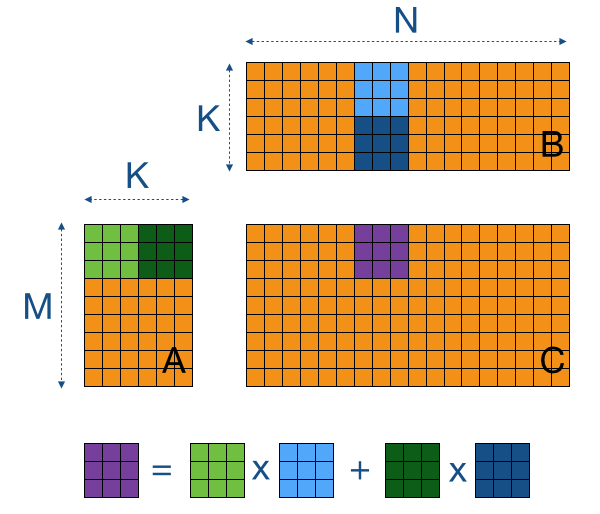
\includegraphics[width=0.50\textwidth]
	{pics/matmul-block1.png}
	\caption{Perkalian matriks per blok.}
	\label{fig:matmulblock}
\end{figure}

Motivasi dari penggunaan blok pada perkalian matriks adalah untuk meningkatkan efisiensi penggunaan cache pada GPU. Perhatikan bahwa untuk mendapatkan suatu elemen baris ke i dan kolom ke j dari matriks, baris ke i dari matriks A dan kolom ke j dari akan diload ke memory dan cache. Kemudian untuk mendapatkan suatu elemen baris ke i+1 dan kolom ke j dari matriks, kolom ke j dari matriks B kembali diload ke memory. Kolom ke j dari matriks B ini selalu digunakan ulang dalam menghitung elemen kolom ke j pada matriks C.

Untuk matriks berukuran besar, besar kemungkinan bahwa kolom tersebut sudah terhapus dari cache karena sebelum memproses kolom itu lagi, cache terlebih dahulu digunakan untuk menyimpan kolom-kolom lain karena sudah banyak perkalian yang dilakukan. Sedangkan ketika matriks berukuran kecil, peluang kolom tersebut masih berada di cache lebih tinggi, sehingga komputasi menggunakan kolom tersebut menjadi lebih cepat. Inilah mengapa matriks dibagi ke dalam beberapa bagian yang lebih kecil untuk dikalikan secara bertahap agar frekuensi penggunaan cache lebih tinggi sehingga komputasi lebih cepat. 

Perkalian per blok ini dapat diimplementasikan dalam OpenCL kernel seperti berikut. Iterasi dilakukan sebanyak K/blocksize kali. Pada setiap iterasi, perkalian per blok dilakukan untuk 32 kolom dari matriks A (semua baris) dan 32 baris dari matriks B (semua kolom). Ingat bahwa ukuran blok adalah 32x32.

\begin{lstlisting}[frame=single]
__kernel void matrixVectorMul(__global float* C, 
const __global float* A, 
const __global float* B, 
int K, int M, int N) { 

// Local row ID (max: 32)
const int row = get_local_id(0);
// Local col ID (max: 32)  
const int col = get_local_id(1);
// Row ID of C (0..M)  
const int globalRow = 32*get_group_id(0) + row; 
// Col ID of C (0..N) 
const int globalCol = 32*get_group_id(1) + col;  

__local float Asub[32][32]; 
__local float Bsub[32][32]; 

float acc = 0.0; 

const int numTiles = ((K-1)/32)+1; 
for (int t=0; t<numTiles; t++) { 

const int tiledRow = 32*t + row; 
const int tiledCol = 32*t + col; 
if((tiledCol < K) && (globalRow < M)) {
Asub[col][row] = A[globalRow*K + tiledCol]; 
}  
else {   
Asub[col][row] = 0.0; 
}  
if((tiledRow < K) && (globalCol < N)) {
Bsub[col][row] = B[globalCol*K + tiledRow]; 
}  
else {   
Bsub[col][row] = 0.0; 
}  

barrier(CLK_LOCAL_MEM_FENCE); 

for (int k=0; k<32; k++) { 
acc += Asub[k][row] * Bsub[col][k]; 
} 

barrier(CLK_LOCAL_MEM_FENCE); 
} 

if((globalRow < M) && (globalCol < N)) { 
C[globalCol*M + globalRow] = acc; 
}
}
\end{lstlisting}

%-----------------------------------------------------------------------------%
\section{Vulkan Matriks Convolution}
%-----------------------------------------------------------------------------%
%-----------------------------------------------------------------------------%
\chapter{\babLima}
%-----------------------------------------------------------------------------%
Bagian ini bersisi pelaksanaan dan hasil eksperimen serta analisis dari hasil tersebut.

%-----------------------------------------------------------------------------%
\section{Mengubah Tampilan Teks}
%-----------------------------------------------------------------------------%


%-----------------------------------------------------------------------------%
\section{Memberikan Catatan}
%-----------------------------------------------------------------------------%


%-----------------------------------------------------------------------------%
\section{Menambah Isi Daftar Isi}
%-----------------------------------------------------------------------------%


%-----------------------------------------------------------------------------%
\section{Memasukan PDF}
%-----------------------------------------------------------------------------%



%-----------------------------------------------------------------------------%
\section{Membuat Perintah Baru}
%-----------------------------------------------------------------------------%


%-----------------------------------------------------------------------------%
\chapter{\babEnam}
%-----------------------------------------------------------------------------%
\todo{tambahkan kata-kata pengantar bab 6 disini}

%---------------------------------------------------------------
\section{Kesimpulan}
%---------------------------------------------------------------


%---------------------------------------------------------------
\section{Saran}
%---------------------------------------------------------------

%
% Daftar Pustaka
%
% Daftar Pustaka 
% 

% 
% Tambahkan pustaka yang digunakan setelah perintah berikut. 
% 
\phantomsection %hack to add clickable section for pustaka
\begin{thebibliography}{4}
\bibitem{openclguide}
{Aaftab Munshi, Benedict Gaster, Timothy G. Mattson, James Fung, and Dan Ginsburg. 2011. OpenCL Programming Guide (1st ed.). Addison-Wesley Professional.}

\bibitem{mobilenet}
{Andrew G. Howard and (2017). MobileNets: Efficient Convolutional Neural Networks for Mobile Vision. CoRR, abs/1704.04861.}

\bibitem{inceptionv3a}
{Christian Szegedy and (2015). Rethinking the Inception Architecture for Computer Vision. CoRR, abs/1512.00567.}

\bibitem{tflite}
{Introduction to TensorFlow Lite | TensorFlow. (n.d.). Retrieved from https://www.tensorflow.org/mobile/tflite/.}

\bibitem{cnndroid}
{Latifi Oskouei, S. S., Golestani, H., Hashemi, M., \& Ghiasi, S. (2016). CNNdroid. In Proceedings of the 2016 ACM on Multimedia Conference - MM ’16. ACM Press. https://doi.org/10.1145/2964284.2973801}

\bibitem{deeplearning}
{Lecun, Y., Bengio, Y., \& Hinton, G. (2015). Deep learning. Nature, 521(7553), 436-444. doi:10.1038/nature14539}

\bibitem{lenet}
{LeCun, Y., Haffner, P., Bottou, L., \& Bengio, Y. (1999). Object Recognition with Gradient-Based Learning. https://doi.org/10.1007/3-540-46805-6\_19.}

\bibitem{tensorflow}
{Martín Abadi, dkk.. TensorFlow: Large-scale machine learning on heterogeneous systems, 2015. Software available from tensorflow.org.}

\bibitem{deeplearningmatrix}
{Michael A. Nielsen, "Neural Networks and Deep Learning", Determination Press, 2015.}

\bibitem{opencl}
{Munshi, A. (2009). The OpenCL specification. 2009 IEEE Hot Chips 21 Symposium (HCS). doi:10.1109/hotchips.2009.7478342}

\bibitem{trainvsinfer}
{NVIDIA White Paper. 2015. GPU-Based Deep Learning Inference: A Performance and Power Analysis}

\bibitem{cnn}
{O'Shea, Keiron \& Nash, Ryan. (2015). An Introduction to Convolutional Neural Networks. ArXiv e-prints.}

\bibitem{lstm}
{Sepp Hochreiter and Jürgen Schmidhuber. 1997. Long Short-Term Memory. Neural Comput. 9, 8 (November 1997), 1735-1780. DOI=http://dx.doi.org/10.1162/neco.1997.9.8.1735
}

\bibitem{inception}
{Szegedy, C., Wei Liu, Yangqing Jia, Sermanet, P., Reed, S., Anguelov, D., … Rabinovich, A. (2015). Going deeper with convolutions. In 2015 IEEE Conference on Computer Vision and Pattern Recognition (CVPR). IEEE. https://doi.org/10.1109/cvpr.2015.7298594}

\bibitem{adrenoopencl}
{Wang, H., Yun, J., \& Bourd, A. (2018). OpenCL Optimization and Best Practices for Qualcomm Adreno GPUs. In Proceedings of the International Workshop on OpenCL - IWOCL ’18. ACM Press. https://doi.org/10.1145/3204919.3204935}

\bibitem{opengl}
{https://www.khronos.org/opengl/}

\bibitem{vulkan}
{https://www.khronos.org/vulkan/}

\bibitem{cnnori}
{Y. Le Cun, B. Boser, J. S. Denker, R. E. Howard, W. Habbard, L. D. Jackel, and D. Henderson. 1990. Handwritten digit recognition with a back-propagation network. In Advances in neural information processing systems 2, David S. Touretzky (Ed.). Morgan Kaufmann Publishers Inc., San Francisco, CA, USA 396-404.}

\end{thebibliography}



%
% Lampiran 
%
\begin{appendix}
	%
% @author  Andreas Febrian
% @version 1.00 
% 
% Hanya sebuah pembatas bertuliskan LAMPIRAN ditengah halaman. 
% 

\begin{titlepage}
	\centering 
	\vspace*{6cm}
	\noindent \Huge{LAMPIRAN}
	\addChapter{LAMPIRAN}
\end{titlepage}
	\setcounter{page}{2}
	%-----------------------------------------------------------------------------%
\addChapter{Lampiran 1}
\chapter*{Lampiran 1}
%-----------------------------------------------------------------------------%
\end{appendix}

\end{document}